\documentclass[a4paper,12pt,twoside]{memoir}

% Castellano
\usepackage[spanish,es-tabla]{babel}
\selectlanguage{spanish}
\usepackage[utf8]{inputenc}
\usepackage[T1]{fontenc}
\usepackage{lmodern} % Scalable font
\usepackage{microtype}
\usepackage{placeins}

\RequirePackage{booktabs}
\RequirePackage[table]{xcolor}
\RequirePackage{xtab}
\RequirePackage{multirow}

% Links
\usepackage[colorlinks]{hyperref}
\hypersetup{
	allcolors = {red}
}

% Ecuaciones
\usepackage{amsmath}

% Rutas de fichero / paquete
\newcommand{\ruta}[1]{{\sffamily #1}}

% Párrafos
\nonzeroparskip


% Imagenes
\usepackage{graphicx}
\newcommand{\imagen}[2]{
	\begin{figure}[!h]
		\centering
		\includegraphics[width=0.9\textwidth]{#1}
		\caption{#2}\label{fig:#1}
	\end{figure}
	\FloatBarrier
}

\newcommand{\imagenflotante}[2]{
	\begin{figure}%[!h]
		\centering
		\includegraphics[width=0.9\textwidth]{#1}
		\caption{#2}\label{fig:#1}
	\end{figure}
}



% El comando \figura nos permite insertar figuras comodamente, y utilizando
% siempre el mismo formato. Los parametros son:
% 1 -> Porcentaje del ancho de página que ocupará la figura (de 0 a 1)
% 2 --> Fichero de la imagen
% 3 --> Texto a pie de imagen
% 4 --> Etiqueta (label) para referencias
% 5 --> Opciones que queramos pasarle al \includegraphics
% 6 --> Opciones de posicionamiento a pasarle a \begin{figure}
\newcommand{\figuraConPosicion}[6]{%
  \setlength{\anchoFloat}{#1\textwidth}%
  \addtolength{\anchoFloat}{-4\fboxsep}%
  \setlength{\anchoFigura}{\anchoFloat}%
  \begin{figure}[#6]
    \begin{center}%
      \Ovalbox{%
        \begin{minipage}{\anchoFloat}%
          \begin{center}%
            \includegraphics[width=\anchoFigura,#5]{#2}%
            \caption{#3}%
            \label{#4}%
          \end{center}%
        \end{minipage}
      }%
    \end{center}%
  \end{figure}%
}

%
% Comando para incluir imágenes en formato apaisado (sin marco).
\newcommand{\figuraApaisadaSinMarco}[5]{%
  \begin{figure}%
    \begin{center}%
    \includegraphics[angle=90,height=#1\textheight,#5]{#2}%
    \caption{#3}%
    \label{#4}%
    \end{center}%
  \end{figure}%
}
% Para las tablas
\newcommand{\otoprule}{\midrule [\heavyrulewidth]}
%
% Nuevo comando para tablas pequeñas (menos de una página).
\newcommand{\tablaSmall}[5]{%
 \begin{table}
  \begin{center}
   \rowcolors {2}{gray!35}{}
   \begin{tabular}{#2}
    \toprule
    #4
    \otoprule
    #5
    \bottomrule
   \end{tabular}
   \caption{#1}
   \label{tabla:#3}
  \end{center}
 \end{table}
}

%
% Nuevo comando para tablas pequeñas (menos de una página).
\newcommand{\tablaSmallSinColores}[5]{%
 \begin{table}[H]
  \begin{center}
   \begin{tabular}{#2}
    \toprule
    #4
    \otoprule
    #5
    \bottomrule
   \end{tabular}
   \caption{#1}
   \label{tabla:#3}
  \end{center}
 \end{table}
}

\newcommand{\tablaApaisadaSmall}[5]{%
\begin{landscape}
  \begin{table}
   \begin{center}
    \rowcolors {2}{gray!35}{}
    \begin{tabular}{#2}
     \toprule
     #4
     \otoprule
     #5
     \bottomrule
    \end{tabular}
    \caption{#1}
    \label{tabla:#3}
   \end{center}
  \end{table}
\end{landscape}
}

%
% Nuevo comando para tablas grandes con cabecera y filas alternas coloreadas en gris.
\newcommand{\tabla}[6]{%
  \begin{center}
    \tablefirsthead{
      \toprule
      #5
      \otoprule
    }
    \tablehead{
      \multicolumn{#3}{l}{\small\sl continúa desde la página anterior}\\
      \toprule
      #5
      \otoprule
    }
    \tabletail{
      \hline
      \multicolumn{#3}{r}{\small\sl continúa en la página siguiente}\\
    }
    \tablelasttail{
      \hline
    }
    \bottomcaption{#1}
    \rowcolors {2}{gray!35}{}
    \begin{xtabular}{#2}
      #6
      \bottomrule
    \end{xtabular}
    \label{tabla:#4}
  \end{center}
}

%
% Nuevo comando para tablas grandes con cabecera.
\newcommand{\tablaSinColores}[6]{%
  \begin{center}
    \tablefirsthead{
      \toprule
      #5
      \otoprule
    }
    \tablehead{
      \multicolumn{#3}{l}{\small\sl continúa desde la página anterior}\\
      \toprule
      #5
      \otoprule
    }
    \tabletail{
      \hline
      \multicolumn{#3}{r}{\small\sl continúa en la página siguiente}\\
    }
    \tablelasttail{
      \hline
    }
    \bottomcaption{#1}
    \begin{xtabular}{#2}
      #6
      \bottomrule
    \end{xtabular}
    \label{tabla:#4}
  \end{center}
}

%
% Nuevo comando para tablas grandes sin cabecera.
\newcommand{\tablaSinCabecera}[5]{%
  \begin{center}
    \tablefirsthead{
      \toprule
    }
    \tablehead{
      \multicolumn{#3}{l}{\small\sl continúa desde la página anterior}\\
      \hline
    }
    \tabletail{
      \hline
      \multicolumn{#3}{r}{\small\sl continúa en la página siguiente}\\
    }
    \tablelasttail{
      \hline
    }
    \bottomcaption{#1}
  \begin{xtabular}{#2}
    #5
   \bottomrule
  \end{xtabular}
  \label{tabla:#4}
  \end{center}
}



\definecolor{cgoLight}{HTML}{EEEEEE}
\definecolor{cgoExtralight}{HTML}{FFFFFF}

%
% Nuevo comando para tablas grandes sin cabecera.
\newcommand{\tablaSinCabeceraConBandas}[5]{%
  \begin{center}
    \tablefirsthead{
      \toprule
    }
    \tablehead{
      \multicolumn{#3}{l}{\small\sl continúa desde la página anterior}\\
      \hline
    }
    \tabletail{
      \hline
      \multicolumn{#3}{r}{\small\sl continúa en la página siguiente}\\
    }
    \tablelasttail{
      \hline
    }
    \bottomcaption{#1}
    \rowcolors[]{1}{cgoExtralight}{cgoLight}

  \begin{xtabular}{#2}
    #5
   \bottomrule
  \end{xtabular}
  \label{tabla:#4}
  \end{center}
}


















\graphicspath{ {./img/} }

% Capítulos
\chapterstyle{bianchi}
\newcommand{\capitulo}[2]{
	\setcounter{chapter}{#1}
	\setcounter{section}{0}
	\chapter*{#2}
	\addcontentsline{toc}{chapter}{#2}
	\markboth{#2}{#2}
}

% Apéndices
\renewcommand{\appendixname}{Apéndice}
\renewcommand*\cftappendixname{\appendixname}

\newcommand{\apendice}[1]{
	%\renewcommand{\thechapter}{A}
	\chapter{#1}
}

\renewcommand*\cftappendixname{\appendixname\ }

% Formato de portada
\makeatletter
\usepackage{xcolor}
\newcommand{\tutor}[1]{\def\@tutor{#1}}
\newcommand{\course}[1]{\def\@course{#1}}
\definecolor{cpardoBox}{HTML}{E6E6FF}
\def\maketitle{
  \null
  \thispagestyle{empty}
  % Cabecera ----------------
\noindent
\includegraphics[width=\textwidth]{cabecera}\vspace{1cm}%
  \vfill
  % Título proyecto y escudo informática ----------------
  \colorbox{cpardoBox}{%
    \begin{minipage}{.8\textwidth}
      \vspace{.5cm}\Large
      \begin{center}
      \textbf{TFG del Grado en Ingeniería Informática}\vspace{.6cm}\\
      \textbf{\LARGE\@title{}}
      \end{center}
      \vspace{.2cm}
    \end{minipage}

  }%
  \hfill\begin{minipage}{.20\textwidth}
    
\includegraphics[width=\textwidth]{escudoInfor}
  \end{minipage}
  \vfill
  % Datos de alumno, curso y tutores ------------------
  \begin{center}%
  {%
    \noindent\LARGE
    Presentado por \@author{}\\ 
    en Universidad de Burgos --- \@date{}\\
    Tutor: \@tutor{}\\
  }%
  \end{center}%
  \null
  \cleardoublepage
  }
\makeatother

\newcommand{\nombre}{Alicia Olivares Gil} %%% cambio de comando

% Datos de portada
\title{título del TFG}
\author{\nombre}
\tutor{Álvar Arnáiz González}
\date{\today}

\begin{document}

\maketitle


\newpage\null\thispagestyle{empty}\newpage


%%%%%%%%%%%%%%%%%%%%%%%%%%%%%%%%%%%%%%%%%%%%%%%%%%%%%%%%%%%%%%%%%%%%%%%%%%%%%%%%%%%%%%%%
\thispagestyle{empty}


\noindent
\includegraphics[width=\textwidth]{cabecera}\vspace{1cm}

\noindent D. Álvar Arnáiz González, profesor del departamento de Ingeniería Civil, área de Lenguajes y Sistemas Informáticos.

\noindent Expone:

\noindent Que el alumno D. \nombre, con DNI dni, ha realizado el Trabajo final de Grado en Ingeniería Informática titulado título de TFG. 

\noindent Y que dicho trabajo ha sido realizado por el alumno bajo la dirección del que suscribe, en virtud de lo cual se autoriza su presentación y defensa.

\begin{center} %\large
En Burgos, {\large \today}
\end{center}

\vfill\vfill\vfill

% Author and supervisor
\begin{minipage}{0.45\textwidth}
\begin{flushleft} %\large
Vº. Bº. del Tutor:\\[2cm]
D. Álvar Arnáiz González
\end{flushleft}
\end{minipage}
\hfill
\begin{minipage}{0.45\textwidth}
\begin{flushleft} %\large
Vº. Bº. del co-tutor:\\[2cm]
D. José Francisco Díez Pastor
\end{flushleft}
\end{minipage}
\hfill

\vfill

% para casos con solo un tutor comentar lo anterior
% y descomentar lo siguiente
%Vº. Bº. del Tutor:\\[2cm]
%D. nombre tutor


\newpage\null\thispagestyle{empty}\newpage




\frontmatter

% Abstract en castellano
\renewcommand*\abstractname{Resumen}
\begin{abstract}
En este primer apartado se hace una \textbf{breve} presentación del tema que se aborda en el proyecto.
\end{abstract}

\renewcommand*\abstractname{Descriptores}
\begin{abstract}
Palabras separadas por comas que identifiquen el contenido del proyecto Ej: servidor web, buscador de vuelos, android \ldots
\end{abstract}

\clearpage

% Abstract en inglés
\renewcommand*\abstractname{Abstract}
\begin{abstract}
A \textbf{brief} presentation of the topic addressed in the project.
\end{abstract}

\renewcommand*\abstractname{Keywords}
\begin{abstract}
keywords separated by commas.
\end{abstract}

\clearpage

% Indices
\tableofcontents

\clearpage

\listoffigures

\clearpage

\listoftables
\clearpage

\mainmatter
\capitulo{1}{Introducción}

Descripción del contenido del trabajo y del estrucutra de la memoria y del resto de materiales entregados.

\capitulo{2}{Objetivos del proyecto}

En este apartado se exponen los objetivos perseguidos con la realización de este trabajo: 

\section{Objetivos generales}

\begin{itemize}
	\item Generar un modelo de clasificación capaz de detectar crisis epilépticas a partir de los datos disponibles. 
	\item Aplicar técnicas de minería de datos siguiendo los pasos del Descubrimiento de Conocimiento en Bases de Datos (\textit{KDD})~\cite{fayyad1996data}.
	\item Investigar sobre técnicas del estado del arte aplicadas a problemas similares. 
	\item Explorar, aplicar y comparar distintas formas de preprocesado de los datos (filtrado, normalización, transformación, etc.). 
	\item Usar técnicas de proyección de datos a dos dimensiones para comprobar si los instancias de <<crisis>> son fácilmente separables de las instancias de <<no crisis>>. 
	\item Probar modelos de clasificación para conjuntos de datos con preprocesados basados en estadísticas simples.
	\item Probar modelos de clasificación para conjuntos de datos con preprocesados basados en características de series temporales.  
	\item Probar modelos de clasificación mediante \textit{ensembles} para conjuntos de datos desequilibrados. 
	\item Probar detección de anomalías mediante un modelo \textit{One-Class}.
	\item Comparar el rendimiento de los modelos obtenidos. 
	\item Comparar distintas métricas usadas para evaluar el rendimiento los modelos obtenidos. 
	\item Desarrollar una app de Android para mostrar la aplicabilidad del modelo de clasificación generado. 
\end{itemize}

\section{Objetivos técnicos}

\begin{itemize}
	\item Aprender \LaTeX{}, en concreto su uso en herramientas de escritorio y online (tales como Overleaf).  
	\item Realizar y exponer los resultados de los experimentos en notebooks de jupyter empleando código Python. 
	\item Usar bibliotecas de minería de datos en Python, en concreto sklearn~\cite{scikit-learn}, para la proyección de los datos y para la obtención y evaluación de los modelos.
	\item Generar un conjunto de transformadores compatibles con sklearn para poder aplicar las técnicas de preprocesado de forma directa.
	\item Utilizar bibliotecas de procesamiento y visualización de datos tales como Pandas y Matplotlib.  
	\item Usar la biblioteca tsfresh~\cite{christ2018time} para extracción de características en series temporales. 
	\item Usar la herramienta Weka~\cite{hall2009weka} para probar modelos de clasificación mediante ensembles en conjuntos de datos desequilibrados. 
	\item Desarrollar una app Android con soporte para API 23 y superiores. 
	\item Usar peticiones HTTP desde la app para la comunicación con la API del servidor remoto. 
	\item Usar Socket.IO desde la app para la obtención de datos en tiempo real del servidor remoto.
	\item Usar la plataforma GitHub junto con la extensión ZenHub para la gestión del proyecto. 
	\item Aplicar la metodología Scrum adaptada a un proyecto con fines educativos. 
	\item Realizar test de sistema y de usabilidad. 
	
	
\end{itemize}

\section{Objetivos personales}

\begin{itemize}
	\item Iniciarme en el campo de la investigación. 
	\item Explorar técnicas y herramientas aplicadas a la minería de datos. 
	\item Aprender a generar documentación con \LaTeX{}. 
	\item Iniciarme en el desarrollo de aplicaciones Android.
	\item Emplear técnicas para abordar un problema real que ayude a las personas con epilepsia crónica.  
\end{itemize}

\capitulo{3}{Conceptos teóricos}\label{conceptos teoricos}

Este proyecto se centra principalmente en investigación, por lo que tiene una importante carga teórica. En el apéndice del cuaderno de investigación se explica el uso de todas las técnicas que hemos empleado en los experimentos, especificando implementaciones concretas, parámetros utilizados y resultados obtenidos. Por otra parte, en este apartado se van a exponer los conceptos teóricos en los que se basan esas técnicas sin entrar en los detalles de implementación.  

Dado que el desarrollo de la investigación se ha basado en el proceso \textit{KDD} (explicado más detenidamente en el apartado de Técnicas y Herramientas), este apartado se estructurará en función de los pasos que incluye este proceso: 

\section{Limpieza de datos}

Los datos de los que disponemos tienen los siguientes atributos: 

\begin{itemize}
	\item \textbf{MAC\_NGMATT} y \textbf{UUID\_BSN}: identificador del colchón asociado alos tubos de presión e identificador del sensor de biométricas respectivamente. 
	\item \textbf{DateTime}: día y hora en la que fue tomada cada instancia de dato. 
	\item \textbf{P1, P2, P3, P4, P5, P6, P7, P8, P9, P10, P11, P12}: presiones, en mBar, captadas por los 12 tubos de presión integrados en el colchón. 
	\item \textbf{HR, RR, SV, HRV, B2B}: valores de las constantes vitales que corresponden con la frecuencia cardíaca (pulsaciones/minuto), la frecuencia respiratoria (respiraciones/minuto), el volumen sistólico (mililitros), la variabilidad del ritmo cardíaco (milisegundos) y el tiempo entre pulsaciones (milisegundos) respectivamente. 
	\item \textbf{SS}: potencia de la señal relativa a la matriz de tubos de presión. Un valor superior a 400 se considera aceptable. 
	\item \textbf{STATUS}: estado de medición del sensor de constantes vitales. 0=\textit{low signal}, 1=\textit{ok signal}, 2=\textit{high signal}, 3= \textit{close to overload}, 4= \textit{close to max HR}. 
\end{itemize}

Por otra parte se nos proporcionaron unos rangos aproximados de horas en los que el paciente tuvo un ataque epiléptico, lo que nos permite etiquetar cada instancia de datos como <<crisis>> o <<no crisis>>.  

\subsection{Eliminación de instancias por baja señal}

Dos de estos atributos, SS y STATUS, hacen referencia a la calidad de la instancia de los datos, uno haciendo referencia a la matriz de tubos de presión y otro al sensor de constantes vitales, y dado que la fase de limpieza de datos consiste en eliminar el ruido y las instancias incorrectas, es aquí donde eliminaremos todas las instancias cuyos datos no consideremos fiables en función de los valores de estos dos atributos. 

\subsection{Eliminación manual del ruido}

Una opción para eliminar el ruido de los datos es hacerlo de forma manual, inspeccionando los datos disponibles y modificando o eliminando aquellos que sean inconsistentes.  

\subsection{Eliminación del ruido mediante filtrado}

Otra forma de eliminar el ruido de una señal consiste en usar filtros. Un filtro es un sistema que se aplica a una señal (en nuestro caso la señal de presiones en el tiempo) y la transforma para conseguir un objetivo concreto, en este caso el suavizado de la señal para eliminar el ruido. Se han probado dos tipos de filtro distintos: 

\begin{itemize}
	\item \textbf{Filtro de Butterworth}~\cite{wiki:butterworth,scipybutter}: Diseñado para filtrado de señales eléctricas, trata de producir la respuesta más plana que sea posible hasta la frecuencia de corte (\textit{Wn}), dicho de otra forma, trata de mantener intactas las frecuencias por debajo de la frecuencia de corte mientras disminuye las frecuencias superiores con razón proporcional a \textit{N}, siendo \textit{N} el orden de filtrado:
	\begin{center}
		$|H| = \dfrac{1}{\sqrt{1+(W/Wn)^{2N}}}$
	\end{center}

	\begin{figure}[H]
		\centering
		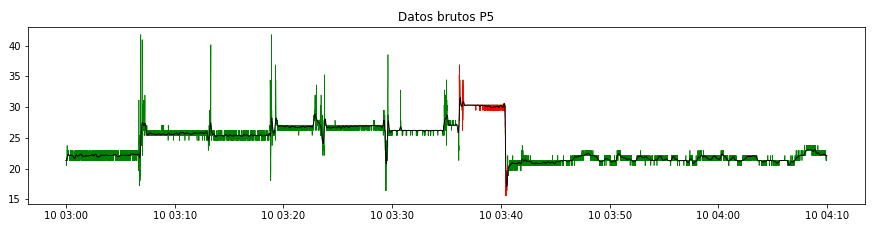
\includegraphics[width=1\textwidth]{../img/senalP5butter.png}
		\caption[Señal de presión (P5) filtrada con Butterworth.] {Ejemplo de señal de presión (P5) filtrada mediante un filtro de Butterworth con \textit{N}=3 y \textit{Wn}=0.05. En verde la señal original y en negro la señal filtrada.}
		\label{fig:senalP5butter}
	\end{figure}
	
	\item \textbf{Filtro de Savitzky–Golay}~\cite{wiki:savitzkygolay,scipysavgol}: Se basa en el cálculo de una regresión polinomial local para la que se debe especificar un tamaño de ventana (\textit{window\_lenght}) y el orden del polinomio utilizado en la regresión (\textit{polyorder}). 
	
	\begin{figure}[H]
		\centering
		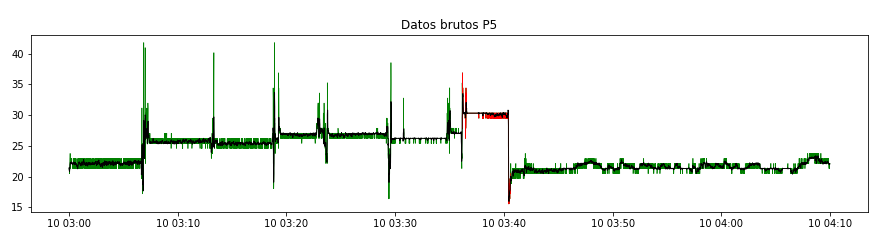
\includegraphics[width=1\textwidth]{../img/senalP5savgol.png}
		\caption[Señal de presión (P5) filtrada con Svatzky-Golay.]{Ejemplo de señal de presión (P5) filtrada mediante un filtro de Svatzky-Golay con \textit{window\_length}=15 y \textit{polyorder}=2. En verde la señal original y en negro la señal filtrada}
		\label{fig:senalP5savgol}
	\end{figure}
\end{itemize}

\subsection{Eliminación de atributos inconsistentes}

Al trabajar con datos reales, cabe la posibilidad de que algunos de los atributos contengan datos inconsistente, ya sea por que se produjeron errores (humanos o sistemáticos) durante la captación de los mismos o porque se corrompieron o perdieron durante su almacenamiento o su envío. Estos datos deberán ser eliminados para no interferir en la fase de minería de datos. Como se explicará en el apartado \ref{aspectos relevantes} de Aspectos Relevantes, en esta fase nos vimos obligados a eliminar los datos relativos a las constantes vitales. 

\section{Integración de datos}

Los datos disponibles corresponden con las instancias recogidas a lo largo de varios meses de una sola cama (un solo paciente). Estos datos nos han sido proporcionados en varios archivos de extensión .csv, por lo que la fase de integración ha consistido en recoger los datos en varios subconjuntos, uno por cada noche, considerando que una noche corresponde con el periodo de tiempo en el que el paciente estuvo acostado en la cama de forma ininterrumpida. 

\section{Selección de datos}

La selección de los datos consiste en desechar aquellos atributos o instancias que no resultan útiles para la extracción de conocimiento. A estas alturas del proceso seguimos teniendo datos relativos a la identificación del colchón, a la hora en la que se tomó la instancia de dato y a las presiones. 

\subsection{Eliminación de identificadores}

Al contar con los datos de un único paciente, los atributos de identificación de la cama MAC\_NGMATT y UUID\_BSN no proporcionan ningún tipo de información útil para la extracción de conocimiento, por lo que ni siquiera son tenidos en cuenta en la fase de integración. 

\subsection{Eliminación de atributos de baja variabilidad}

Este proceso consiste en detectar aquellos atributos que varían menos de un umbral determinado durante el tiempo, y por lo tanto no proporcionarán información relevante. Como se explicará en el apartado \ref{aspectos relevantes} de Aspectos relevantes, este proceso nos llevó a desechar la mitad de los datos relativos a los tubos de presión. 

En este punto ya hemos seleccionado los atributos que serán considerados como \textbf{Datos en Bruto}: DateTime, P1, P2, P3, P4, P5 y P6.

\subsection{Selección de atributos para el entrenamiento}

Tras la fase de transformación de datos, la cual se abordará a continuación, se contará con una gran cantidad atributos calculados a partir de los datos en bruto. En la mayoría de los casos, resulta más eficiente entrenar el modelo de clasificación solo con un subconjunto de ellos que proporcione la mayor imformación, y por ello es necesario plantear estrategias para seleccionar el mejor subconjunto. En este proyecto se han planteado dos estrategias distintas: 

\begin{itemize}
	\item Escoger los atributos mejor situados en un ranking elaborado en función del rendimiento del clasificador en base a una métrica de evaluación concreta (estos conceptos se explican en fases posteriores). 
	\item Emplear un algoritmo genético para encontrar el mejor subconjunto de atributos. 
\end{itemize}

\subsubsection{Algoritmo genético}

Un algoritmo genético~\cite{koza92} es un método iterativo de búsqueda y optimización inspirado en la evolución biológica y el mecanismo de selección natural. En el contexto de un algoritmo genético una posible solución del problema se denomina <<individuo>>, y en cada iteración el algoritmo trabajará con un conjunto de individuos llamado <<población>> o <<generación>>. Los individuos tienen dos tipos de representación: 
\begin{itemize}
	\item \textbf{El genotipo:} es la representación del individuo que se empleará en las operaciones de cruce y mutación. 
	\item \textbf{El fenotipo:} es la representación del individuo que se empleará en la operación de evaluación. 
\end{itemize}

En cada iteración (o generación) se llevarán a cabo 4 operaciones: 
\begin{enumerate}
	\item \textbf{Selección} de los mejores individuos de la generación en base a una función de evaluación, que en nuestro caso se basará en el rendimiento de un clasificador entrenado con los atributos indicados por el individuo. 
	\item \textbf{Cruce} de algunos de los mejores individuos generando otros nuevos mediante la combinación de sus genotipos. 
	\item\textbf{Mutación} de algunos de los mejores individuos generando otros nuevos mediante la modificación de una pequeña parte de sus genotipos.
	\item \textbf{Reemplazo} de los individuos de la anterior generación por los nuevos individuos generados.  
\end{enumerate}

Cada uno de estos pasos puede emplear distintos mecanismos o implementaciones en función del genotipo de los individuos, el tipo de problema y otras consideraciones a tener en cuenta. 

\section{Transformación de datos}

\subsection{Técnicas de reducción de la dimensionalidad}

El primer tipo de transformación de datos que se utilizó fueron las técnicas de reducción de dimensionalidad~\cite{fodor2002dimreduction}. Estas técnicas consisten en proyectar datos en un plano, reduciendo su dimensión (número de atributos de cada instancia, en nuestro caso seis) a dos. Este tipo de enfoques se basan en la hipótesis de que la dimensionalidad de los conjuntos de datos es artificialmente alta, y que se puede mantener la misma información con una representación de los mismos con una dimensionalidad menor. 

\begin{figure}[H]
	\centering
	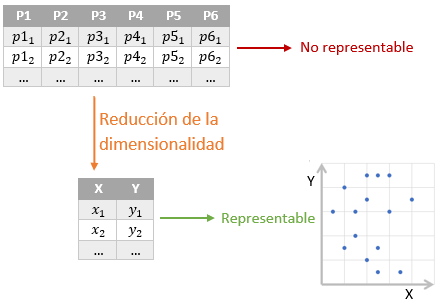
\includegraphics[width=0.7\textwidth]{../img/reducdim.png}
	\caption{Abstracción de la reducción de la dimensionalidad de los datos.}
	\label{fig:reducdim}
\end{figure}


Con esto, el objetivo que se persiguió fue comprobar si las instancias de <<crisis>> eran fácilmente separables de las instancias de <<no crisis>> en una representación bidimensional de los datos. Existen varios tipos de técnicas, cada una basada en unos criterios concretos para realizar la proyección, y se pueden clasificar principalmente en transformaciones lineales y transformaciones no lineales.  

\subsubsection{Transformaciones lineales}

Este tipo de transformaciones supone que los datos observados son combinación lineal de una cierta base, y en ellas se engloba el \textbf{Análisis de Componentes Principales} (\textit{PCA})~\cite{pca}. 

\textit{PCA} es una de las técnicas más utilizadas y consiste en escoger el nuevo sistema de coordenadas (o base) de forma que se maximice la varianza entre las instancias. Cabe destacar que para el nuevo sistema de coordenadas se puede escoger cualquier dimensionalidad menor o igual a la del conjunto original de datos. Sin embargo, a mayor dimensionalidad, mayor coste de computación, y no es posible representar en papel proyecciones de más de 2 dimensiones, por lo que solo se ha probado esta última. 

\begin{figure}[H]
	\centering
	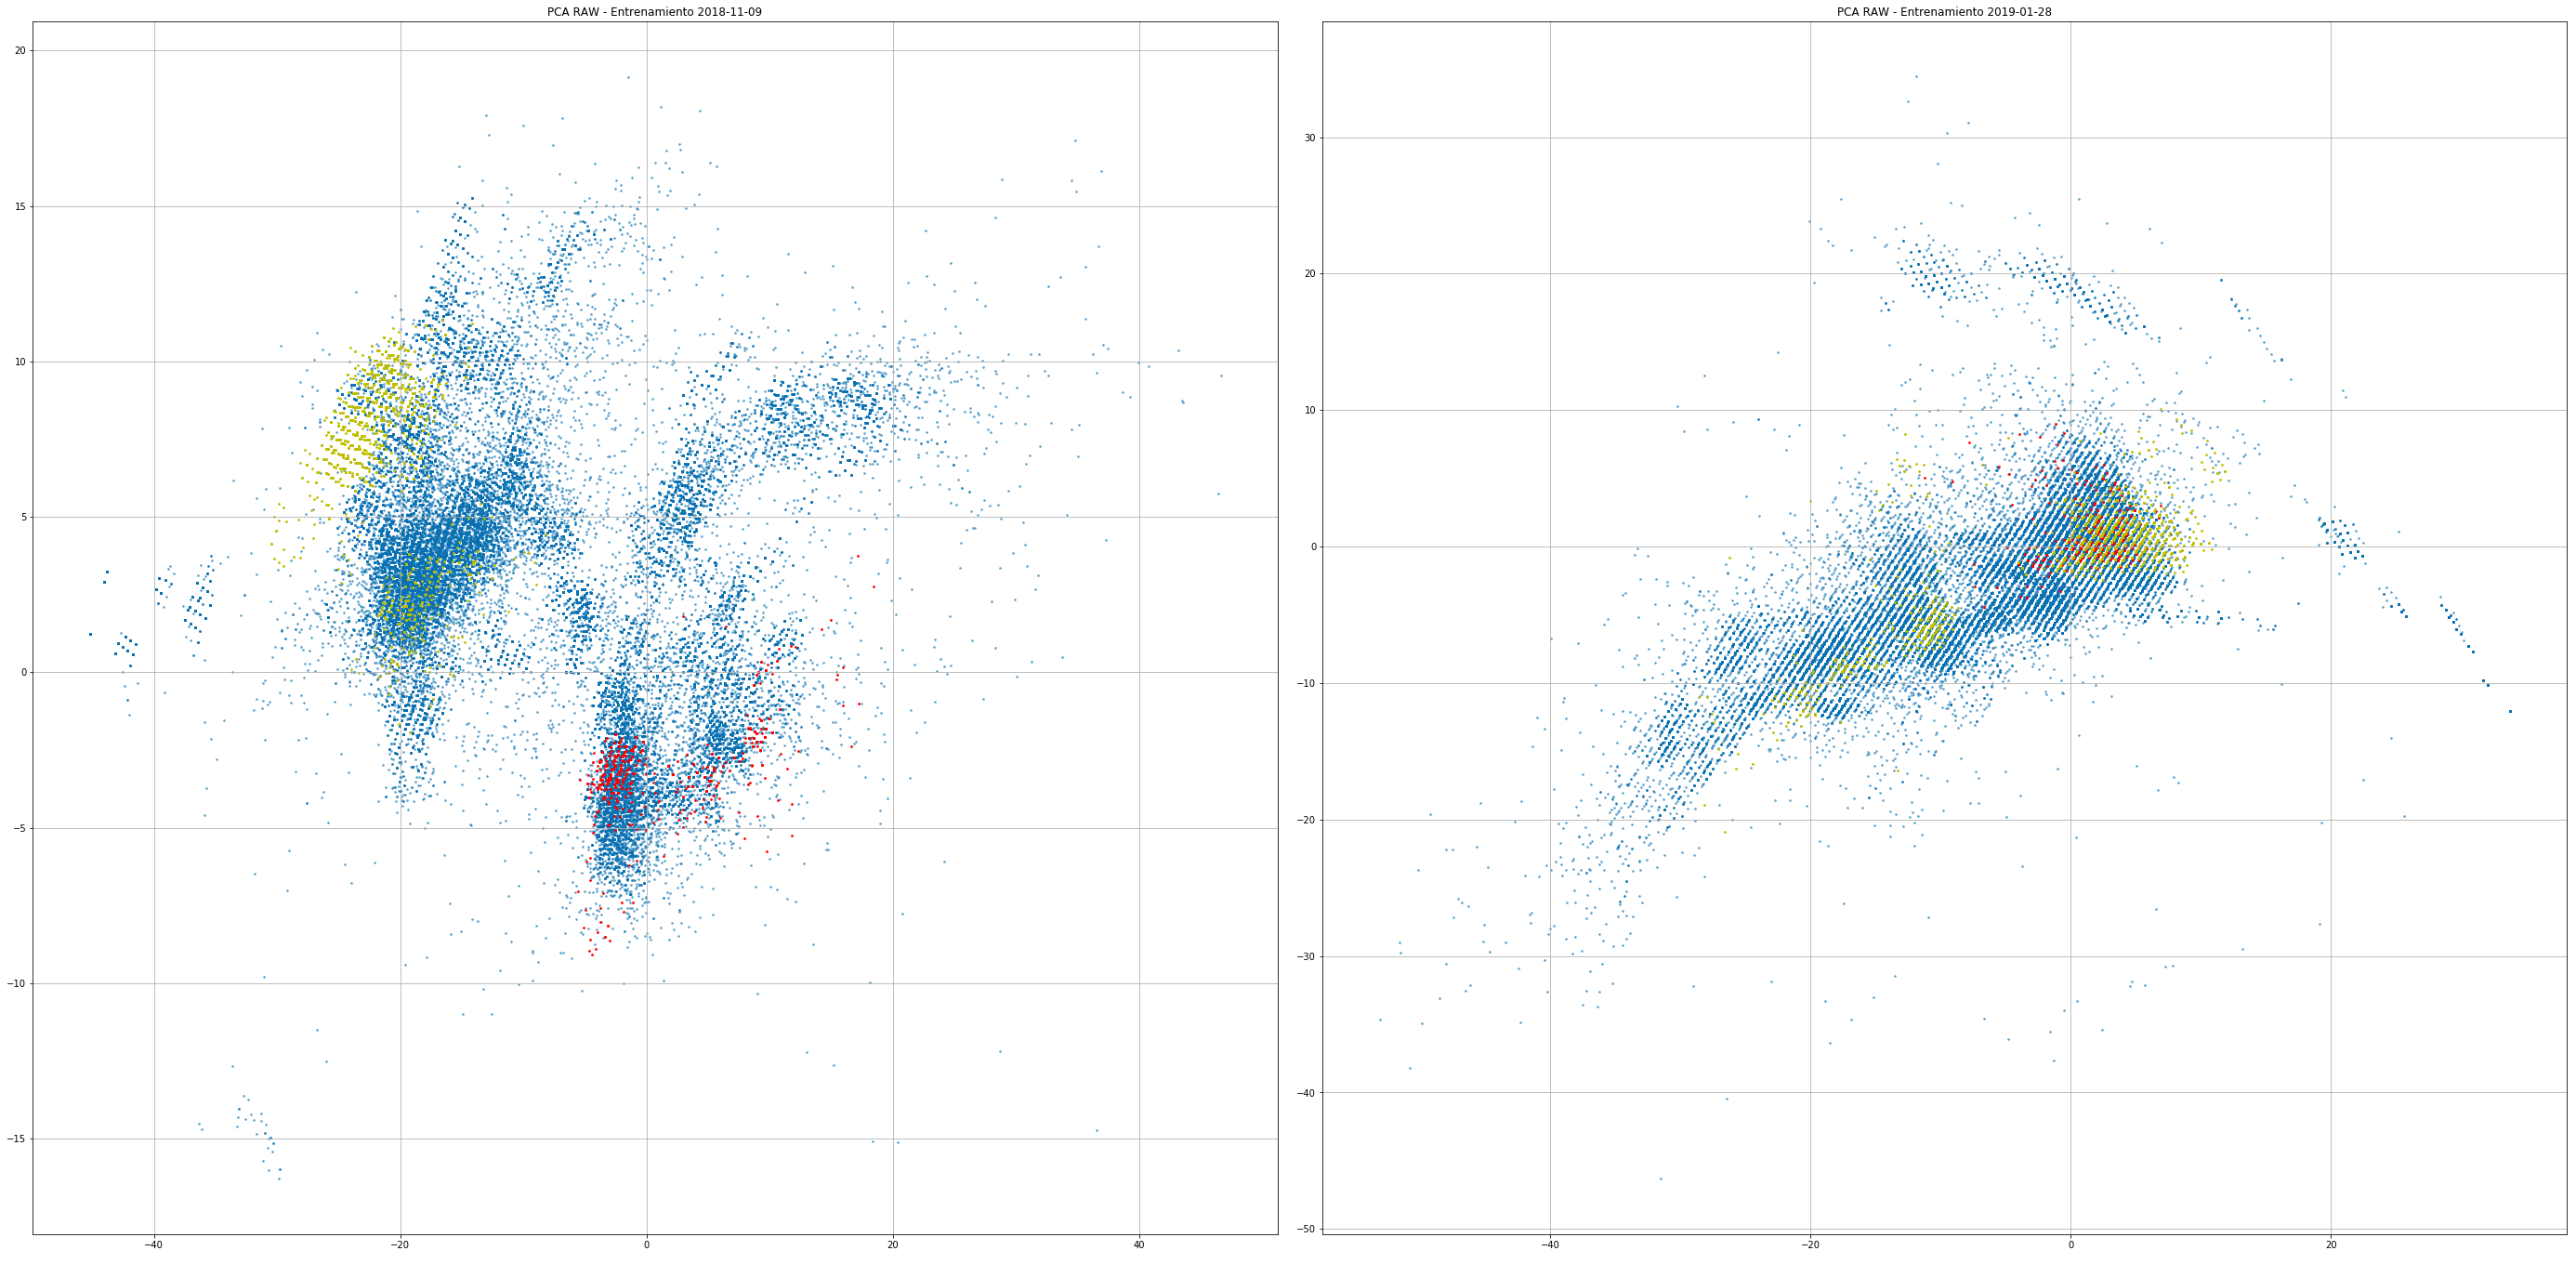
\includegraphics[width=1\textwidth]{../img/pca.png}
	\caption[Ejemplo de \textit{PCA}.] {\textit{PCA} aplicado a la noche de la crisis 1 (izquierda) y a la noche de la crisis 2 (derecha).}
	\label{fig:pca}
\end{figure}

En la figura~\ref{fig:pca} los puntos rojos corresponden con instancias de <<crisis>> y los azules con instancias de <<no crisis>>. Como se puede ver no existe separación entre ellas. Los puntos amarillos corresponden con instancias de la otra crisis, y se puede ver que tampoco comparten espacio. 

\subsubsection{Transformaciones no lineales}

Las transformaciones no lineales~\cite{manifold}, no asumen que los datos sean una combinación lineal de una base. Existen varias técnicas de este tipo y en nuestro caso se han probado con éxito las siguientes: 

\begin{itemize}
	\item \textbf{\textit{Isomap}~\cite{isomap}:} Trata de reducir la dimensionalidad manteniendo las distancias geodésicas entre todas las instancias.
	\item \textbf{\textit{Locally Linear Embedding} (\textit{LLE})~\cite{lle}:} Reduce la dimensionalidad preservando las distancias dentro de los <<vecindarios>> locales. Se puede considerar como un conjunto de \textit{PCA}s locales que se comparan globalmente para encontrar la mejor reducción no lineal. 
	\item \textbf{\textit{Multi-Dimensional Scaling} (\textit{MDS}):~\cite{mds}} Es una técnica bastante utilizada en marketing y ciencias sociales que se basa en la similitud o disimilitud de los datos. Busca reducir la dimensionalidad tratando las distancias como valores proporcionales a la disimilitud de las instancias (lo que se parecen entre ellas).   
\end{itemize}

\begin{figure}
	\centering
	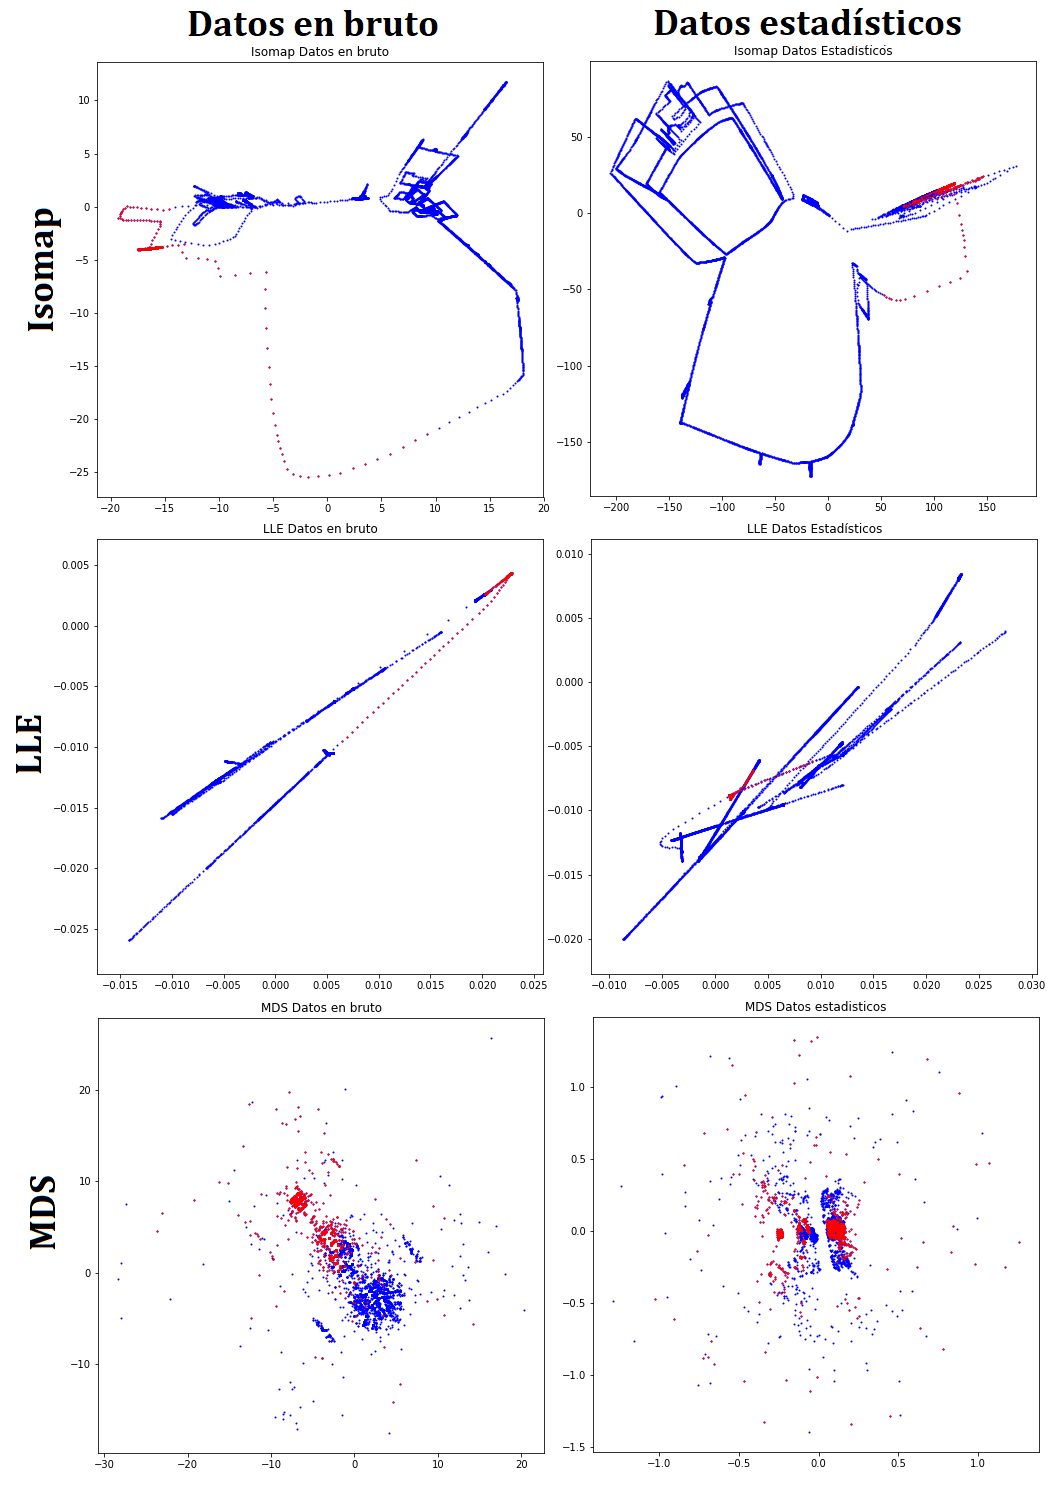
\includegraphics[width=1\textwidth]{../img/manifolds.png}
	\caption{Comparativa de las técnicas de transformación no lineal.}
	\label{fig:manifolds}
\end{figure}

Como se aprecia en la figura~\ref{fig:manifolds} con algunas de estas técnicas se consigue un grado algo mayor de separación, pero las instancias siguen sin ser fácilmente separables. En este caso, y como se puede observar, hemos aplicado las técnicas no solo a los datos en bruto sino también a los datos estadísticos, lo que nos lleva al siguiente tipo de transformación. 

\subsection{Cálculo de estadísticas móviles}

Las técnicas de minería de datos se pueden aplicar directamente a los datos en bruto, pero en ocasiones ofrecen un mejor rendimiento aplicadas a datos estadísticos calculados a partir de estos. Para calcular estadísticas móviles se debe definir el tamaño de la ventana (\textit{N}), de forma que para cada ventana se calculará un valor estadístico a partir de los datos contenidos en ella. Se han usado tres estadísticas simples: 

\begin{minipage}{\linewidth}
\begin{itemize}
	\item \textbf{Media móvil:} Es el valor promedio de los valores contenidos en la ventana. 
	\begin{center}
		$ \overline{x}=\frac{1}{N}\sum_{i=1}^{N}x_{i}$
	\end{center}
	\item \textbf{Desviación típica móvil:} Es una medida de la dispersión de los valores contenidos en la ventana. 
	\begin{center}
		$ \sigma=\sqrt{\frac{1}{N-1}\sum_{i=1}^{N}(x_{i}-\overline{x})^2}$
	\end{center}
	\item \textbf{Rango móvil:} Es la diferencia entre el valor máximo y el valor mínimo de los contenidos en la ventana. 
\end{itemize}
\end{minipage}

\subsection{Cálculo de características de series temporales}

Además de las descritas en el apartado anterior, se pueden calcular multitud de estadísticas más complejas, como es el caso de las características de series temporales. 

Una serie temporal~\cite{wiki:serietemporal} no es más que una secuencia de instancias medidas en determinado momento de tiempo y ordenadas cronológicamente, por lo que nuestro conjunto de datos corresponde con la definición de serie temporal. Las series temporales se suelen usar para estudiar la relación causal entre diversas variables que cambian en el tiempo y pueden influirse entre sí. Para este cometido existen una serie de técnicas específicas basadas en cálculos estadísticos más complejos. 

Para este proyecto se ha empleado la biblioteca tsfresh~\cite{christ2018time} que extrae algunas de esas características a partir de una serie temporal, y hemos tratado de usarlas para generar el modelo de clasificación. 

\section{Minería de datos}

En esta fase se ha tratado de generar un modelo capaz de encontrar los patrones que definen una crisis epiléptica. Para ello el modelo debe ser capaz de aprender a partir de los datos, y en función de como lo haga se puede hablar de dos tipos básicos de aprendizaje: supervisado y no supervisado. 

\begin{itemize}
	\item Un modelo de \textbf{aprendizaje supervisado} se entrena con un conjunto de datos etiquetado, es decir, que cada instancia de dato de entrenamiento tiene asociado un valor categórico que ofrece información sobre a qué clase pertenece (para un problema de clasificación) o un valor nominal (para un problema de regresión). Este es un problema de clasificación y las dos clases posibles son <<crisis>> o <<no crisis>>. Tras el entrenamiento, el modelo deberá ser capaz de etiquetar nuevas instancias de dato distintas a las que se han usado en el entrenamiento como instancias de <<crisis>> o <<no crisis>> basándose en lo aprendido. En definitiva, el ciclo de vida de un clasificador supervisado tiene dos fases: 
	\begin{enumerate}
		\item \textbf{Entrenamiento:} El modelo aprende a partir de un conjunto de datos etiquetado. 
		\item \textbf{Predicción:} El modelo predice la clase de un dato no etiquetado, es decir, cuya clase real se desconoce. 
	\end{enumerate}
	
	\item En el \textbf{aprendizaje no supervisado} el modelo no tiene conocimiento sobre a qué clase pertenece cada instancia. Con este tipo de aprendizaje se pueden, por ejemplo, agrupar los datos en subconjuntos en función de sus características. Las técnicas de reducción de la dimensionalidad podrían ser consideradas técnicas de aprendizaje no supervisado, ya que elaboran la proyección sin conocer la clase de cada instancia, pero podrían darnos información sobre la existencia de dos clases si en las proyecciones bidimensionales existiera una clara separación entre dos grupos (\textit{clusters}) de instancias. 
\end{itemize}

Por otra parte, dentro de los modelos de clasificación podemos distinguir entre clasificadores simples o \textit{ensembles}.

\begin{itemize}
	\item Los \textbf{clasificadores simples} emplean un solo modelo que será el encargado de predecir la clase de las nuevas instancias. 
	\item Los \textbf{\textit{ensembles}}~\cite{kuncheva2004combining} son conjuntos de clasificadores simples cuyas predicciones se combinan para obtener una predicción final. La idea es construir varios modelos que no necesariamente predigan la misma clase para la misma instancia, y será la combinación de estas predicciones, por ejemplo, mediante votación, la que determinará la clase que predice el \textit{ensemble}. Para que este sistema de clasificación tenga sentido los modelos que forman el \textit{ensemble} deben ser algo distintos entre sí, de lo contrario no ofrecerían ninguna ventaja, y esa diferencia puede radicar en varios mecanismos, por ejemplo: 
	\begin{itemize}
		\item El proceso de construcción del modelo no es determinista, por lo que al entrenar varias instancias de ese modelo no se generan clasificadores exactamente iguales. 
		\item El \textit{ensemble} se compone de modelos obtenidos con distintos métodos, llamados métodos heterogéneos. 
		\item Cada modelo se entrena con un conjunto de datos diferente.
		\item Cada modelo se entrena con un subconjunto de atributos diferente para el conjunto de datos. 
	\end{itemize} 
\end{itemize} 

\begin{figure}[H]
	\centering
	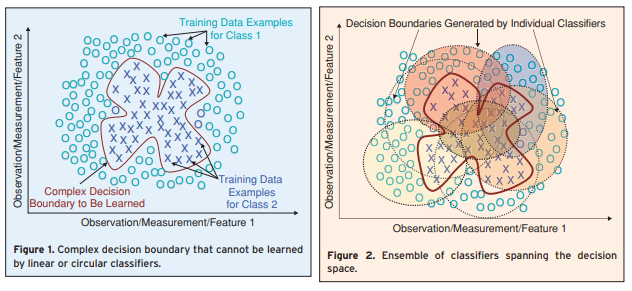
\includegraphics[width=1\textwidth]{../img/ensembles.png}
	\caption[Uso de \textit{ensembles} para problemas de clasificación complejos.]{Uso de \textit{ensembles} para problemas de clasificación complejos~\cite{polikar2006ensemble}.}
	\label{fig:ensemble}
\end{figure}

Teniendo en cuenta estas distinciones a continuación se exponen los modelos de clasificación que se han probado en este proyecto.

\subsection{Random Forest}

El clasificador \textit{Random Forest} es un \textit{ensemble} que emplea  árboles de decisión, y se trata de uno de los más sencillos y utilizados. Para construir cada árbol emplea la técnica de \textit{Bagging}, que consiste en entrenar cada modelo con un conjunto de datos del mismo tamaño que el original pero generado mediante muestreo uniforme con reemplazo (los datos pueden aparecer varias veces en el mismo conjunto). Mediante este mecanismo se reduce la varianza y se evita el sobreajuste. 

Además, durante la construcción de los árboles que componen el \textit{ensemble}, en cada nodo de decisión se tendrá en cuenta únicamente un subconjunto aleatorio de atributos del conjunto de datos.

Dado que todos los modelos del \textit{ensemble} son independientes los unos de los otros, tienen la misma importancia, por lo que su voto tendrá el mismo peso a la hora de calcular la predicción final. 

\subsection{One-Class}

La detección de anomalías One-Class consiste en entrenar el modelo con instancias de una sola clase de forma que a la hora evaluar nuevas instancias, devolverá información sobre si cada una pertenece o no a la clase basándose, de alguna forma, en su similitud con las instancias usadas en el entrenamiento. 

Por ejemplo, si entrenamos el clasificador solo con instancias etiquetadas como <<no crisis>> y utilizamos datos de ambas clases para la predicción, esta puede devolver dos valores: 

\begin{minipage}{\linewidth}
\begin{itemize}
	\item La nueva instancia corresponde con la clase, por lo que se predice <<no crisis>>. 
	\item La nueva instancia no corresponde con la clase, por lo que se predice <<crisis>>. 
\end{itemize}
\end{minipage}

Durante el entrenamiento no se indica explícitamente a qué clase pertenece cada instancia, pero dado que todas las instancias de entrenamiento pertenecen a la misma, sí se le está proporcionando cierta información sobre la clase a la que pertenecen, y por lo tanto puede ser considerado como un algoritmo de aprendizaje supervisado. 

\subsection{AdaBoost.M1}

Se trata de un \textit{ensemble} para clasificación multi-clase que emplea aprendizaje supervisado. Emplea el método de \textit{Boosting}, que a diferencia de \textit{Bagging} es iterativo, y genera cada modelo del \textit{ensemble} influenciado por el rendimiento del anterior. En este caso se busca que cada modelo dé más importancia a las instancias que son mal clasificadas por el modelo anterior. A diferencia de \textit{Bagging} este mecanismo puede producir sobreajuste, sobre todo si el conjunto de datos tiene demasiado ruido. 

Debido a la forma en la que se construyen los modelos simples que lo componen, a la hora de calcular la predicción final para una nueva instancia el voto de cada modelo tendrá un peso distinto en función de su precisión.  

\begin{figure}[H]
	\centering
	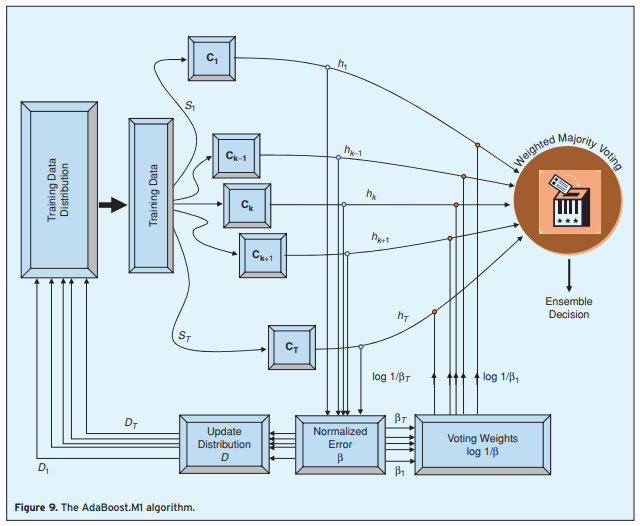
\includegraphics[width=0.8\textwidth]{../img/adaboostm1.png}
	\caption[Funcionamiento del algoritmo AdaBoost.M1.]{Funcionamiento del algoritmo AdaBoost.M1~\cite{polikar2006ensemble}.}
	\label{fig:adaboostm1}
\end{figure}

\subsection{Rotation Forest}

\textit{Rotation Forest}~\cite{rodriguez2006rotation} es también un \textit{ensemble} para clasificación que emplea aprendizaje supervisado mediante árboles de decisión. No se basa en un algoritmo iterativo como \textit{Boosting}, por lo que los clasificadores simples pueden ser generados de forma paralela. Se trata de un método algo más complejo que los anteriores, basado en la aplicación del ya mencionado \textit{PCA} a subconjuntos, preferiblemente disjuntos, de atributos. Además, al igual que en \textit{Bagging}, cada árbol se entrena con conjuntos de datos construidos mediante muestreo con reemplazo a partir del conjunto original. 

\section{Evaluación de patrones}

En el contexto de este trabajo, la utilidad de los patrones encontrados corresponderá con la precisión del clasificador en sus predicciones. Dado que al clasificar instancias nuevas no conocemos a priori la clase a la que pertenecen, no podemos saber si la clasificación ha sido correcta, por lo que para calcular la precisión de un clasificador se debe usar una partición de entrenamiento y test del conjunto original de datos disponibles: 

\begin{minipage}{\linewidth}
\begin{itemize}
	\item La \textbf{partición de entrenamiento} contiene la mayoría de los datos (por ejemplo, el 75\%), los cuales serán usados para entrenar el clasificador. 
	\item El resto corresponden con la \textbf{partición de test}, que serán usados para comparar su clase real (su etiqueta) con la clase predicha por el clasificador entrenado.
\end{itemize} 
\end{minipage} 

La precisión corresponde con el porcentaje de acierto del clasificador para la partición de entrenamiento, pero en ocasiones, conviene usar métricas más complejas para medir el rendimiento de un clasificador. En este trabajo se ha trabajado con dos métricas distintas: el área bajo la curva ROC y la precisión media, pero antes de explicarlos es necesario presentar algunos conceptos básicos.  

En un problema de clasificación binaria como este, si consideramos una instancia de <<crisis>> como un positivo (P) y una instancia de <<no crisis>> como un negativo (N) podemos definir los siguientes valores: 

\begin{itemize}
	\item Verdaderos positivos (VP): número de instancias de <<crisis>> que son clasificadas como <<crisis>>. 
	\item Falsos positivos (FP): número de instancias de <<no crisis>> que son clasificadas como <<crisis>>. 
	\item Verdaderos negativos (VN): número de instancias de <<no crisis>> que son clasificadas como <<no crisis>>. 
	\item Falsos negativos (FN): número de instancias de <<crisis>> que son clasificadas como <<no crisis>>.  
\end{itemize}

Estos valores se suelen visualizar en forma de matriz de confusión, la cual tiene la estructura de la figura~\ref{fig:matrizconfusion}.

\begin{figure}[H]
	\centering
	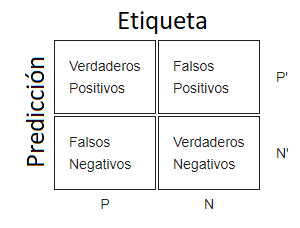
\includegraphics[width=0.5\textwidth]{../img/matrizconfusion.png}
	\caption[Disposición de la matriz de confusión.]{Disposición de la matriz de confusión~\cite{wiki:roc}.}
	\label{fig:matrizconfusion}
\end{figure}  

\subsection{Área bajo la curva ROC (\textit{AUC})}

A partir de los valores anteriores se pueden calcular los siguientes: 

\begin{itemize}
	\item \textbf{Sensibilidad o Razón de Verdaderos Positivos (VPR):}
	\begin{center}
		$VPR=\frac{VP}{P}=\frac{VP}{(VP+FN)}$ 
	\end{center} 
	\item \textbf{Razón de Falsos positivos (FPR):} 
	\begin{center}
		$VPR=\frac{VP}{P}=\frac{VP}{(VP+FN)}$ 
	\end{center} 
\end{itemize}

Algunos clasificadores binarios, como los que se usan en este trabajo, además de predecir la etiqueta de la clase a la que creen que pertenece la instancia, son capaces de devolver la probabilidad entre 0 y 1 de que la instancia pertenezca a esa clase. Usando estas probabilidades podríamos clasificar las instancias en función de un umbral, por ejemplo, una instancia sería considerada <<crisis>> si la probabilidad de que pertenezca a esa clase es mayor o igual a 0.8 y <<no crisis>> si es menor. 

El área bajo la curva ROC (\textit{Receiver Operating Characteristic}) representa la relación entre la VPR y la FPR según se varía ese umbral. Se representará la VPR en el eje $y$, y FPR en el eje $x$. Cada punto corresponderá con los valores VPR y FPR resultantes de escoger cada uno de los posibles umbrales de clasificación, y la unión de esos puntos será lo que llamamos la curva ROC del clasificador.

Nos interesa que el VPR ($sensibilidad$) sea lo mayor posible y que el FPR ($1-especificidad$) sea lo menor posible, por lo que el clasificador óptimo corresponderá con aquel que presenta un área bajo la curva ROC (AUC) igual a 1, mientras que el peor clasificador será aquel con un AUC igual a 0.5, ya que ofrecería una predicción equivalente a lanzar una moneda al aire. 

\begin{figure}[H]
	\centering
	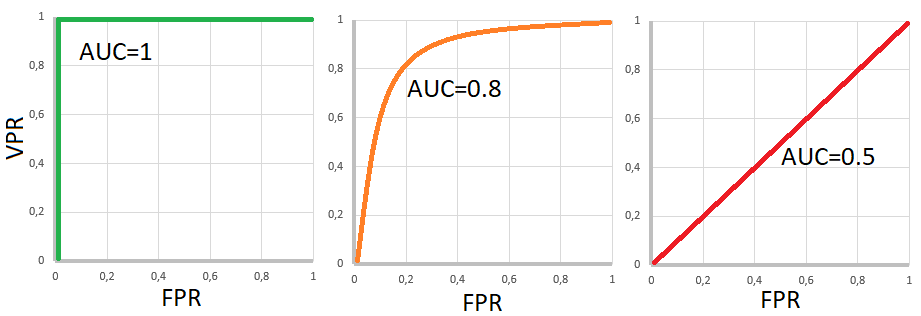
\includegraphics[width=0.7\textwidth]{../img/roc.png}
	\caption{ROC. De izquierda a derecha: mejor caso, caso intermedio y peor caso.}
	\label{fig:roc}
\end{figure} 

\subsection{Precisión media}

Se definen las siguientes variables: 
\begin{center}
	$Precision=\frac{VP}{VP+FP}$
\end{center}
\begin{center}
	$Recall=\frac{VP}{VP+FN}$
\end{center}

La precisión media (AV)~\cite{precisionrecall} se define como lo siguiente: 

\begin{center}
	$AV=\sum_{i=1}^{n}(Recall_{i}-Recall_{i-1})Precission_{i}$
\end{center}

\noindent donde $Precission_{i}$ y $Recall_{i}$ son los valores de \textit{Precision} y \textit{Recall} calculados para el umbral de clasificación i-ésimo, y \textit{n} el número de posibles umbrales. Cuanto mayor sea este valor, mejor se considera el clasificador. 

\section{Presentación del conocimiento}

En este caso una posible presentación útil del conocimiento adquirido sería la representación de la probabilidad de pertenencia a la clase <<crisis>> de cada instancia ordenadas cronológicamente, es decir, cómo varía la probabilidad de crisis epiléptica del paciente con el tiempo en función del modelo. Esta será una de las gráficas que serán visibles en la aplicación de Android desarrollada. 

\begin{figure}[H]
	\centering
	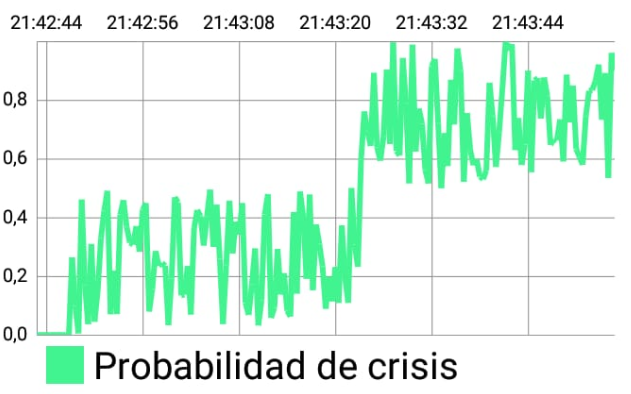
\includegraphics[width=0.7\textwidth]{../img/prob.png}
	\caption{Ejemplo de representación de la probabilidad de crisis en función del tiempo.}
	\label{fig:prob}
\end{figure} 


\capitulo{4}{Técnicas y herramientas}\label{tecnicas y herramientas}

En este apartado se presentan las técnicas metodológicas y las herramientas que se han usado en las distintas fases del desarrollo del proyecto. 


\section{Técnicas metodológicas}

\subsection{Scrum}

Como se explica más detenidamente en el apartado de Planificación temporal del Apéndice A, para la planificación y desarrollo del proyecto se ha utilizado la metodología ágil \textit{Scrum}, manteniendo el enfoque incremental de los \textit{sprints} pero adaptándola al contexto de un trabajo con fines educativos. 

\subsection{KDD}

En la fase de investigación se ha seguido el proceso de Descubrimiento de Conocimiento en Bases de Datos o \textit{KDD}~\cite{fayyad1996data}, dedicado a encontrar un modelo válido y útil en la medida en la que sirva para describir los patrones subyacentes de los datos. El término \textit{KDD} suele ser empleado a menudo como sinónimo de minería de datos, pero esta corresponde en realidad con uno solo de los pasos del proceso. Se suele hablar de las siguientes fases englobados en el proceso de \textit{KDD}: 

\begin{itemize}
	\item \textbf{Obtención de datos:} Consiste en recolectar los datos que se van a usar para tratar de obtener conocimiento. 
	\item \textbf{Limpieza de datos:} Consiste en eliminar los datos inconsistentes o con ruido.  
	\item \textbf{Integración de datos:} Se integran los datos de todas las fuentes disponibles en un formato uniforme y adecuado para los pasos posteriores. 
	\item \textbf{Selección de datos:} Se trata de seleccionar solo aquellos datos relevantes para la tarea de análisis.  
	\item \textbf{Transformación de datos:} Se realizan transformaciones y cálculos a partir de los datos en bruto con el fin de aplicar las técnicas de minería a las formas más apropiadas de los mismos. 
	\item \textbf{Minería de datos:} Aplicación de técnicas para encontrar patrones subyacentes. 
	\item \textbf{Evaluación de patrones:} Se estudia hasta qué punto los patrones encontrados son interesantes. 
	\item \textbf{Presentación del conocimiento:} Consiste en ofrecer una representación comprensible y útil de los patrones y del conocimiento extraído. 
\end{itemize}

Estos pasos no se aplican necesariamente de forma secuencial, ya que en muchos casos conviene volver a pasos anteriores tras la evaluación de los resultados del paso actual. 

\section{Herramientas en la fase de investigación}

\subsection{Anaconda}

Anaconda es un administrador de paquetes y de entornos considerado un estándar para el desarrollo de minería de datos en lenguajes como Python y R. Al instalar Anaconda se tienen automáticamente disponibles más de 200 paquetes, además de ofrecer la posibilidad de añadir nuevos de forma sencilla. 

Licencia: \textit{Modified BSD License}

\subsection{Jupyter Notebook}

Los experimentos se han desarrollado en código Python distribuído en múltiples jupyter notebooks, ya que ofrecen un formato de estructuración y documentación del código muy adecuado para la investigación. \textit{Jupyter Notebook} se encuentra disponible al instalar Anaconda. 

Licencia: \textit{Modified BSD License}


\subsection{Scikit-Learn}

Es la principal biblioteca empleada en la fase de investigación. Incluye modelos de clasificación, predicción y clustering de todo tipo y herramientas para entrenarlos, explotarlos y evaluarlos de forma sencilla. Está especialmente diseñada para operar con las bibliotecas \textit{NumPy} y \textit{SciPy}, y es compatible con \textit{Pandas}.

Licencia: \textit{Modified BSD License } 

\subsection{Weka}

En algunas partes de la investigación se han usado modelos de Weka, otra plataforma para aprendizaje automático y minería de datos escrita en Java. Fue utilizada sobre todo para el entrenamiento de \textit{ensembles} aplicados a conjuntos de datos desequilibrados.

Licencia: \textit{GNU General Public License}

\subsection{tsfresh}

Es una biblioteca de Python dedicada al cálculo de grandes cantidades de características de series temporales. Permite calcular 64 tipos distintos de características y dispone de herramientas para filtrarlas en función de su relevancia. Es compatible con \textit{Pandas}. 

Licencia: \textit{MIT License }

\subsection{DEAP}

Es el framework de python para computación evolutiva más utilizado. Se ha empleado como una de las alternativas para intentar encontrar la mejor selección de características de series temporales mediante un algoritmo genético, esperando que al aplicar este conjunto en la fase de minería se obtuviesen los mejores resultados posibles.  

Licencia: \textit{GNU Lesser General Public License v3.0}

\subsection{tmux}

Se trata un multiplexador de terminales que permite abrir varias sesiones simultáneamente y dejarlas corriendo en segundo plano. Esta herramienta ha resultado especialmente útil para la ejecución de los experimentos más costosos en cuanto a tiempo de ejecución. Debido a que las ejecuciones de los experimentos se han llevado a cabo sobre un equipo de cómputo del grupo de investigación de los tutores mediante una conexión ssh que a menudo se cerraba en medio de un trabajo, ha sido necesario abrir una sesión de tmux en el equipo para cada una de estas ejecuciones de forma que, aunque se perdiera la conexión, el proceso siguiera corriendo en segundo plano y pudiéramos acceder a los resultados reactivando la sesión cuando el trabajo finalizase.

Licencia: \textit{Zero clause BSD License}

\subsection{Otras bibliotecas relevantes}
\begin{itemize}
	\item \textit{NumPy} y \textit{Pandas} para la gestión, modificación y presentación de los datos. 
	\item \textit{Matplotlib} para la presentación gráfica de los resultados. 
	\item \textit{pickle} para la serialización de los datos y los resultados de los experimentos. 
\end{itemize}

\section{Herramientas en la fase de diseño de la aplicación}

\subsection{StarUML}

Software de edición de diagramas UML utilizado en la fase de modelado. 

Licencia: Propietaria aunque dispone de una demo gratuíta. 

\subsection{Material Design}

Es una guía de estilo desarrollada por Google e integrada a partir de la versión \textit{Lollipop} (5.0) de Android. Esta guía de estilos trata los elementos de la interfaz como elementos matariales, con unas dimensiones y una posición definida dentro del espacio (no solo en el plano, también en una tercera dimensión representada mediante el atributo \textit{elevation}), propone una serie de dimensiones idóneas para cada tipo de elemento (textos, botones, tarjetas, etc.), y define la forma de generar el esquema de colores de la interfaz.

\subsection{Pencil}

Software de prototipado de interfaces gráficas. Permite incluir paquetes para incorporar elementos propios de \textit{Material Design} a los prototipos, por lo que proporciona una visión más próxima al aspecto final de las interfaces de la aplicación que otros tipos de prototipado. 

Licencia: \textit{GNU Public License version 2} 

\section{Herramientas en la fase de desarrollo de la aplicación}

\subsection{Android Studio}

Es el entorno de desarrollo integrado oficial de Android, disponible para Windows, GNU/Linux y MacOS. Android Studio incluye, entre otras muchas cosas, un editor de código, un editor gráfico de \textit{layouts}, emuladores para todas las versiones de Android existentes, y soporte para construcción automática con Gradle. 

Licencia: \textit{Apache License 2.0}

\subsection{Gradle}

Herramienta para la automatización de la construcción del software para proyectos Java. Es la herramienta soportada de forma oficial por Android.

Licencia: \textit{Apache License 2.0} 

\subsection{Android Support Library}

Es la biblioteca que gestiona la compatibilidad de funciones de versiones avanzadas con su equivalente en versiones anteriores de Android. Además, incluye \textit{layouts}, elementos y utilidades que no están disponibles en el framework oficial. Aunque la biblioteca recomendada actualmente para este cometido es \textit{AndroidX}, la cual incluye las mismas funcionalidades y algunas más, se ha escogido \textit{Android Support Library} por su simplicidad y por su documentación clara y completa, lo que resulta de mucha utilidad cuando se desarrolla una aplicación Android por primera vez. 

Licencia: \textit{Apache License 2.0}

\subsection{MPAndroidChart}

Es una biblioteca para generación de gráficos en aplicaciones Android. En este caso, y aunque no está pensada para ello, se ha utilizado para visualizar gráficas dinámicas cuyos datos se modifican en tiempo real. Para implementar esta funcionalidad se tuvo en cuenta también la biblioteca SciChart, al ser la biblioteca de referencia para generación de gráficos en tiempo real de Android, pero se descartó al tratarse de un software de pago. 

Licencia: \textit{Apache License 2.0}

\subsection{Socket.IO-client Library}

Es una biblioteca para gestión de comunicación mediante sockets para Java. El uso de esta biblioteca viene impuesto por la implementación de la API del servidor remoto, que gestiona el envío de datos en tiempo real de esta forma. 

Licencia: \textit{MIT License}

\subsection{JUnit}

Es un \textit{framework} para generar pruebas unitarias en Java que evalúen si los métodos de nuestras clases muestran el funcionamiento que se espera. JUnit está totalmente integrado en Android Studio. 

Licencia: \textit{Common Public License} 

\subsection{Espresso}

Es una herramienta de grabación de pruebas sobre la UI integrada en Android Studio. Permite grabar las acciones del usuario sobre la interfaz de la aplicación y hacer comprobaciones del contenido tras cada una de las acciones. 

\section{Otras herramientas generales}

\begin{itemize}
	\item \textbf{Git} como sistema de control de versiones distribuido. 
	\item \textbf{GitHub} como plataforma para el \textit{hosting} del repositorio del proyecto. 
	\item \textbf{ZenHub} como extensión de GitHub para la gestión del proyecto basada en la metodología \textit{Scrum}. 
	\item \textbf{GitKraken} como cliente de Git mediante interfaz gráfica. (\textit{GNU Public License}).
	\item \textbf{Overleaf} como editor colaborativo de \LaTeX{} online para la generación del cuaderno de investigación conjunto. 
	\item \textbf{\TeX studio} como editor de \LaTeX{} para la generación de la memoria y los anexos. (\textit{GNU General Public License v2}).
	\item \textbf{FileZilla} como aplicación para transferencia de ficheros. Soporta los protocolos FTP, SFTP y FTPS. (\textit{GNU General Public License v2}).
\end{itemize}





















\capitulo{5}{Aspectos relevantes del desarrollo del proyecto}\label{aspectos relevantes}

En este apartado se presentarán los aspectos relevantes del desarrollo del proyecto, exponiendo los problemas y las principales decisiones tomadas en cada una de las fases. Se distinguirá, de nuevo, entre la fase de investigación y la fase de desarrollo de la aplicación de Android. 

\section{Fase de invstigación}

A continuación se expondrán las distintas situaciones que obligaron a tomar decisiones sobre cómo proseguir con la investigación y se explicará la razón por la que se tomó cada decisión concreta. También se hablará de detalles de implementación que fueron necesarios para abordar algunos de esos problemas. 

Cabe destacar que la fase de investigación se hizo de forma conjunta con mi compañero de proyecto José Luis Garrido Labrador, y que las decisiones se tomaron entre los dos y con la ayuda de nuestros tutores. 

\subsection{Exploración del estado del arte}

Como en cualquier proyecto de investigación, el paso inicial consistió en realizar una exploración del estado del arte sobre métodos y técnicas empleados para la detección automática de ataque epilépticos o de otros problemas similares, como la detección de caídas. En esta exploración se encontró que aunque la detección automática de ataques epilépticos es un campo muy explorado, la mayoría de las técnicas que se encuentran se basan en el uso de Electroencefalogramas (EEG) y pulseras inteligentes basadas en la monitorización de las constantes vitales. Por otro lado, no se encontraron artículos relativos a técnicas o metodologías de aprendizaje a partir de los datos de sensores de presión instalados en colchones o similares.

Por otro lado, dado que el conjunto de datos disponibles es claramente desequilibrado (se tienen muchas más instancias de <<no crisis>> que de <<crisis>>) también se realizó una búsqueda de técnicas aplicadas a este tipo de problemas, lo que nos llevó a los modelos de clasificación expuestos en el apartado~\ref{conceptos teoricos} de Conceptos teóricos. 

\subsection{Etiquetado de los datos}

Uno de los principales problemas que se tuvo que afrontar fue el del etiquetado de los datos, ya que, aunque los proveedores de los datos indicaron también un rango de horas en los que supuestamente tuvo lugar una crisis epiléptica, estos rangos eran muy aproximados y demasiado amplios para lo que dura una crisis epiléptica, según la bibliografía, sin que se produzcan consecuencias fatales o irreversibles. 

Esto nos obligó a realizar una inspección visual de los datos, y ajustar los tiempos de la crisis teniendo en cuenta: 

\begin{itemize}
	\item Los rangos de horas proporcionados por los proveedores de los datos. 
	\item Información relativa al aspecto de las señales en entornos próximos al inicio y final de esos rangos. 
	\item Información relativa a las proyecciones obtenidas mediante las técnicas de reducción de la dimensionalidad, de forma que, si existía algún tipo de separación, se aplicaron las etiquetas de <<crisis>> a solamente aquellas instancias dentro de los rangos que mostraban una separación más clara con las instancias de <<no crisis>>. 
\end{itemize}

\begin{figure}
	\centering
	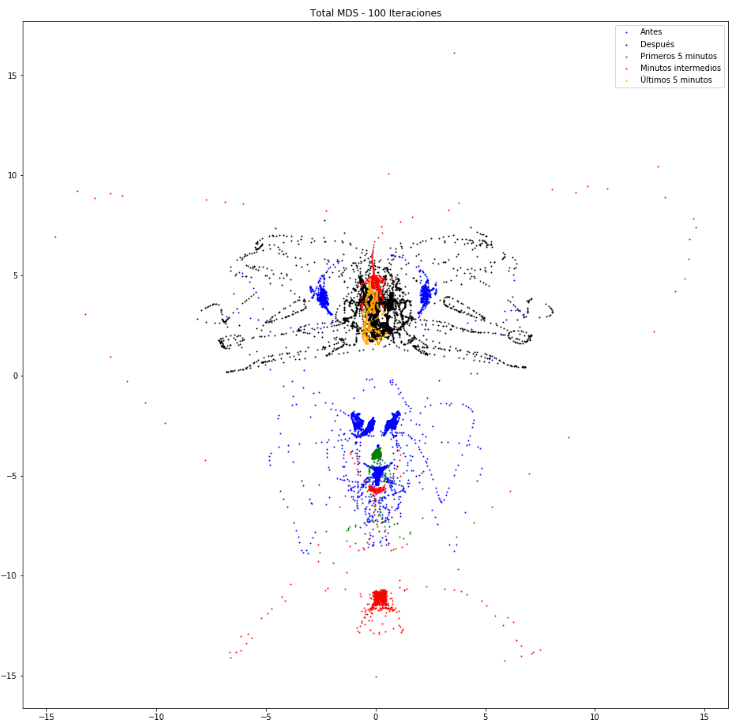
\includegraphics[width=0.7\textwidth]{../img/mdsetiquetado.png}
	\caption{Aplicación de \textit{MDS} para el etiquetado de la primera crisis.}
	\label{fig:mdsetiquetado}
\end{figure}

En la figura~\ref{fig:mdsetiquetado} se muestra la aplicación de la técnica de transformación MDS para el etiquetado de la primera crisis. Las instancias se han dividido en colores en función de su instante de tiempo respecto al rango proporcionado por los proveedores de los datos. Azul: antes de la crisis, Negro: después de la crisis, Verde: primeros 5 minutos de la crisis, Rojo: minutos centrales de la crisis, Naranja: últimos 5 minutos de la crisis. Como se puede observar, las instancias rojas presentan una separación mucho mayor con el resto, y además coinciden con aquellas cuyas señales de presión mostraban una diferencia más significativa dentro de su entorno, por lo que esas fueron las instancias etiquetadas como <<crisis>>. 

Se debe tener en cuenta que, aunque se realizaron estos ajustes, el etiquetado de los datos no puede ser considerado otra cosa que aproximado, y se asume que por esta razón los datos tendrán cierto grado de ruido. Este motivo junto con la escasez de datos de <<crisis>> en el conjunto de datos disponible, representan los mayores problemas a los que me he tenido que enfrentar en el proyecto. 

\subsection{Limpieza de datos}

Del total de datos, hubo que desechar muchas de las instancias por distintas razones. En primer lugar se eliminaron aquellas instancias cuya señal era de mala calidad. Concretamente eliminamos todas aquellas instancias con un SS menor de 400 (como recomendaban los proveedores de los datos), pero no tuvimos en cuenta el valor de STATUS ya que, como se explicará más adelante, los valores de las constantes vitales no se usaron para la búsqueda del modelo de clasificación.

Por otra parte, mediante una inspección inicial de los datos se detectó que algunos datos de los tubos de presión en ocasiones eran negativos (lo cual no debería ocurrir), y aparecían valores bajos de presión en momentos en los que la cama debería estar vacía. Por esta razón, se decidió considerar todo valor de presión menor a 5 como ruido convirtiéndolo automáticamente a 0. De esta forma nos deshicimos también de los valores negativos. Para eliminar el ruido del resto de los datos se aplicó un filtro de Butterworth.

En esta inspección también se advirtió que los atributos referentes a las constantes vitales eran nulos de forma intermitente y en una gran cantidad de las instancias. Como supimos más adelante, esto se debió al mal funcionamiento del sensor durante las primeras etapas de recogida de los datos. Aunque algunas técnicas de minería de datos soportan la presencia de atributos desconocidos (\textit{missing}) en algunas de las instancias, la cantidad de instancias con constantes vitales nulas o incorrectas era tan grande que se tomó la decisión de no tener en cuenta estos datos para el resto de experimentos. Cabe destacar que esto supone un gran inconveniente, ya que la mayoría de técnicas de detección automática encontrados en el estado del arte (quitando las centradas en EEG) se basan en datos biométricos. 

\subsection{Selección de atributos}

A continuación se detectaron los datos con baja variabilidad para su eliminación. Tras llevar a cabo este proceso se eliminaron los atributos P7, P8, P9, P10, P11 y P12. Esto tiene sentido ya que esos campos corresponden con la matriz de tubos de presión de una de las mitades del modelo de colchón de matrimonio, y el colchón con el que se trabaja en este proyecto es individual. Por esta razón eliminar estos datos no supone ninguna pérdida de información, y además, reduce a la mitad la cantidad de datos con la que deben tratar los modelos, lo que repercute positivamente en los tiempos. 

\subsection{Transformadores}

Una vez seleccionado el abanico de operaciones que íbamos a tener en cuenta para la búsqueda de un preprocesado óptimo, se codificaron estas operaciones como transformadores compatibles con sklearn para poder aplicarlas de forma sencilla y sistemática. Para ello se generaron una serie de clases que heredaban la clase \texttt{sklearn.base.TransformerMixin}. En total se codificaron 9 transformadores. 


\subsection{Elección del tamaño de ventana}

Como se ha comentado en el apartado~\ref{conceptos teoricos} de Conceptos teóricos, para calcular estadísticas móviles del conjunto de datos debemos escoger un tamaño de ventana. Para determinar el valor óptimo para este problema, se realizó un barrido de tamaños aplicados a la media y la desviación móviles, datos que se usaron para entrenar y testear un clasificador \textit{Random Forest}. El proceso que se siguió se explica también con detenimiento y detalle en el cuaderno de investigación. 

Para calcular las estadísticas móviles durante la exploración se usó nuestro transformador \texttt{StatisticsTransformer} que utiliza internamente las funciones  \texttt{df.rolling(window\_length).mean()} o \texttt{.std()} según el caso, donde \texttt{df} es el \texttt{pandas.DataFrame} que contiene los datos originales. Esta función devuelve un nuevo \texttt{pandas.DataFrame} con las estadísticas móviles calculadas para cada una de las ventanas (una fila por cada desplazamiento de la ventana). De esta forma, nos evita ir desplazando la ventana manualmente mediante un bucle. 

\begin{figure}[H]
	\centering
	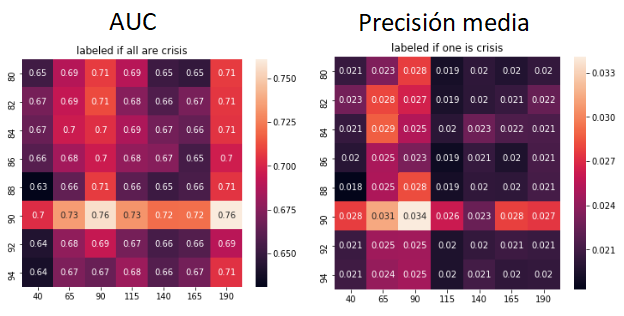
\includegraphics[width=1\textwidth]{../img/heatmap.png}
	\caption[Mapa de calor de los resultados finales de la exploración para cada uno de las métricas de evaluación.]{Mapa de calor de los resultados finales de la exploración para cada uno de las métricas de evaluación. En el eje $y$ el tamaño de la ventana para la desviación típica, en el eje $x$ el tamaño para la media.}
	\label{fig:heatmap}
\end{figure}

Para cada una de las métricas de evaluación del clasificador (AUC y Precisión media) se hicieron una serie de barridos de parámetros, centrándose cada vez más en los rangos en los que se lograba un mejor rendimiento, y llegando finalmente a los resultados que se muestran en la figura~\ref{fig:heatmap}. Como se puede observar, los mejores valores se lograron para un tamaño de ventana de 90 tanto para la desviación típica como para la media, y también para ambas métricas de evaluación. Por esta razón se usó este valor en los experimentos y también como tamaño de ventana para la extracción de características de series temporales. 

\subsection{Extracción de características de series temporales para una ventana de datos}

La extracción de características de series temporales aplicada a un cierto tamaño de ventana no es tan sencilla y merece un comentario sobre cómo se ha resuelto. La función encargada de la extracción de características pertenece la biblioteca \texttt{tsfresh} y se llama \texttt{extract\_features}. Esta función recibe un \texttt{pandas.DataFrame} como parámetro y devuelve una fila de características por cada grupo de filas con el mismo <<id>> (debemos añadir un atributo <<id>> a nuestro conjunto de datos en bruto). Puedes indicarle mediante un diccionario pasado como parámetro el conjunto de características concreto que se desea calcular, o por el contrario, hacer que calcule todo su repertorio de características. Esta misma biblioteca ofrece una función llamada \texttt{utilities.dataframe\_functions.roll\_time\_series()} que, a efectos prácticos, permite la extracción de características aplicada a una ventana, pero lo hace con un coste de memoria tan grande que no resulta práctica para conjuntos de datos como el nuestro. Básicamente, crea un \texttt{pandas.DataFrame} con un <<id>> distinto para cada ventana. Pongamos un ejemplo para comprender su funcionamiento: si tenemos un conjunto de datos con 10 filas y queremos aplicar una ventana de tamaño 3, esta función devuelve: 
\begin{itemize}
	\item 3 filas correspondientes a las filas 1, 2, y 3 del conjunto original y con un <<id>>=1. 
	\item 3 filas correspondientes a las filas 2, 3, y 4 del conjunto original y con un <<id>>=2. 
	\item así sucesivamente. 
\end{itemize}

\begin{figure}[H]
	\centering
	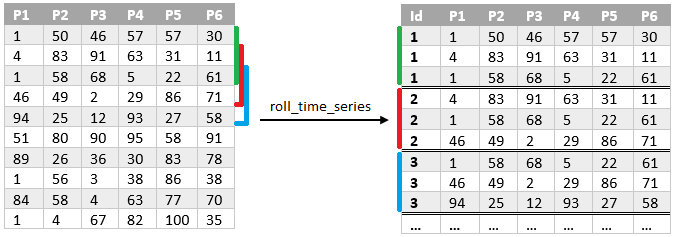
\includegraphics[width=1\textwidth]{../img/rolltimeseries.png}
	\caption{Ejemplo del funcionamiento de la función \texttt{roll\_time\_series}}
	\label{fig:rolltimeseries}
\end{figure}

Por cómo funciona en relación al atributo <<id>>, si aplicamos este nuevo conjunto de datos a la función \texttt{extract\_features} obtenemos lo que buscamos, una fila de características por cada ventana, pero el coste computacional y de memoria que supone la generación de este nuevo conjunto, que tiene una enorme cantidad de datos repetidos, es tan alto que no resulta viable. Por ello, en lugar de usar esta función, se tomó la decisión de realizar el desplazamiento de la ventana de forma manual mediante un bucle.


\subsection{Filtrado de características de series temporales}

Al ejecutar la extracción de características de las datos de las dos noches en las que tuvo lugar una crisis epiléptica, obtenemos 4\,764 características en total, 794 por cada tubo de presión. Este número de atributos es excesivo para aplicarlo directamente a un clasificador, por lo que planteamos varias estrategias para quedarnos con aquellos que aporten mayor información. Estas estrategias se encuentran recogidas y explicadas en el cuaderno de investigación, por lo que aquí se expone la que, por presentar un mejor rendimiento, se empleó como entrada a métodos de selección posteriores. 

Este filtrado consistió en usar la función \texttt{select\_features} de la biblioteca tsfresh, que realiza una selección supervisada de las características (recibe el el valor de las etiquetas de cada instancia). Al aplicar esta función el número de características se redujo a 1\,731. Además, asumimos que una característica solo sería relevante si resulta relevante para todos los tubos de presión, por lo que eliminamos aquellas que, tras el filtrado, no permanecieran para todos los tubos, quedándonos únicamente con 744 (124 para cada tubo de presión).  

\subsection{Selección final de características mediante algoritmo genético}

Una vez filtradas las características más relevantes, es decir, que aportan más información, el último paso consiste en seleccionar un subconjunto más pequeño de ellas que sea suficiente para lograr un buen rendimiento del clasificador. De nuevo, se plantearon varias estrategias cuyo desarrollo se puede consultar en el cuaderno de investigación, y aquí se expondrá la que obtuvo un mejor rendimiento. 

Esta estrategia es la que emplea un algoritmo genético implementado mediante la biblioteca DEAP. Una de las decisiones que hay que tomar a la hora de diseñar un algoritmo genético es qué tipo de genotipo se va a utilizar. En este caso se decidió que el genotipo sería un array unidimensional en el que cada gen (cada posición del array) contiene un número entero entre 0 y 123, que hace referencia a cada una de las 124 características resultantes del filtrado. El tamaño de este array corresponderá con el tamaño máximo de características que pueden ser seleccionadas, y se tomó la decisión de restringir este valor a únicamente 10 características, para que fuera cual fuera el tipo de clasificador escogido finalmente, la clasificación fuese rápida. Esto es importante ya que, en teoría, debe aplicarse a un sistema de recepción de datos en tiempo real. 

\begin{figure}[H]
	\centering
	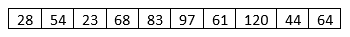
\includegraphics[width=0.7\textwidth]{../img/genotipo.png}
	\caption{Genotipo del mejor individuo encontrado usando el AUC como métrica de evaluación.}
	\label{fig:genotipo}
\end{figure}

Se aclara que 10 es el tamaño \textbf{máximo} de características porque, debido a los mecanismos de mutación y cruce utilizados, una característica puede aparecer más de una vez en un mismo individuo, en cuyo caso solo se tendría en cuenta una vez. Esta decisión se tomó porque de los mecanismos de cruce y mutación que ofrece DEAP, ninguno está preparado para trabajar con pseudopermutaciones (permutaciones en las que el tamaño del array no corresponde con el número de valores que puede contener). Aunque en DEAP es posible crear mecanismos de cruce y mutación personalizados que resolverían este problema, el beneficio que se obtiene con ello es mínimo o nulo. Esto se debe a que al tratar de maximizar el rendimiento, prevalecerán aquellos individuos que aporten mayor información al clasificar, es decir, aquellos con un mayor número de características.

Esto nos lleva a la decisión de cómo implementar la función de adaptación. Como ya hemos comentado, tenemos características relativas a dos noches en las que tuvo lugar una crisis epiléptica, y queremos realizar una evaluación lo más dura posible para que estemos seguros de que el clasificador vaya a predecir bien nuevas instancias. Por esta razón decidimos que la evaluación de los individuos se realizará mediante validación cruzada entre dos días (este tipo de evaluación se usó a menudo en otras fases de la investigación): 

\begin{minipage}{\linewidth}
\begin{enumerate}
	\item Se entrena un clasificador \textit{Random Forest} con las características indicadas por el genotipo del individuo, pero solo con los datos pertenecientes a la noche de la primera crisis. 
	\item Se calcula el rendimiento del clasificador de acuerdo a la métrica pertinente (se usó tanto el AUC como la Precisión media) tomando los datos pertenecientes a la noche de la segunda crisis como partición de test. 
	\item Se realiza el proceso inverso. 
	\item La función de adaptación devolverá la media de los dos rendimientos obtenidos, el cual se tratará de maximizar. 
\end{enumerate}
\end{minipage}

Las últimas decisiones que se deben tomar en relación a la configuración del algoritmo son el tamaño de la población y el número de generaciones que se ejecutan. En ambos casos se escoge un valor de 50 teniendo en cuenta lo costosa que es la evaluación de cada individuo, y se confirma la decisión al ver que tras la ejecución se observa que no se producen mejoras en las últimas generaciones. 

\begin{figure}
	\centering
	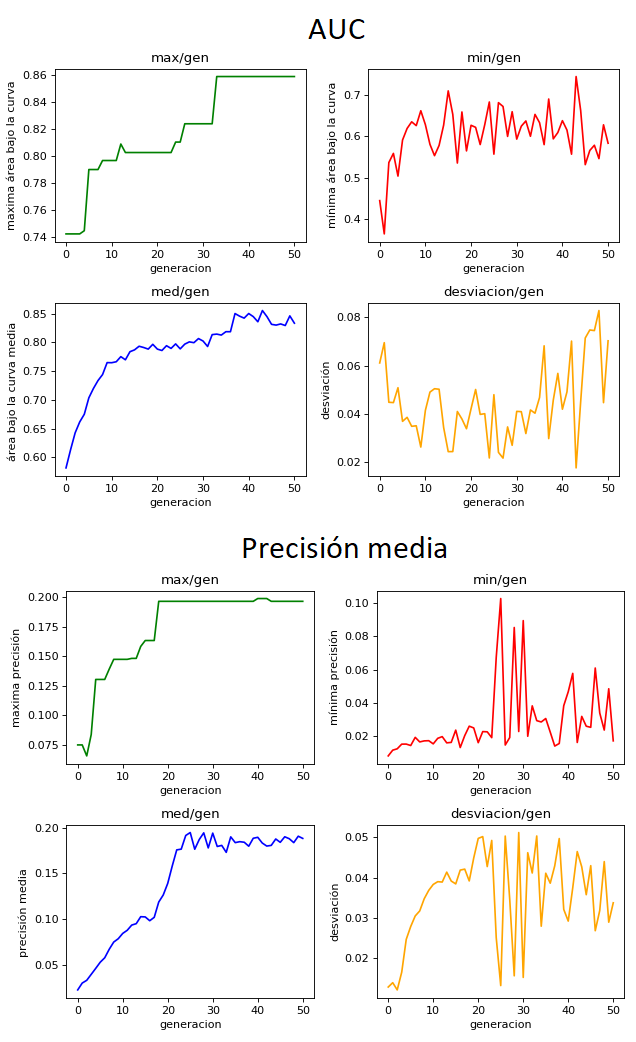
\includegraphics[width=0.8\textwidth]{../img/genetico.png}
	\caption{Evolución del algoritmo genético para cada una de las métricas de evaluación consideradas.}
	\label{fig:genetico}
\end{figure}

\subsection{One-Class y \textit{ensembles} para desequilibrados}

Las características seleccionadas mediante el algoritmo genético no se probaron unicamente en un clasificador \textit{Random Forest}, también se probaron en otros de los clasificadores comentados en el apartado~\ref{conceptos teoricos} de Conceptos teóricos. Sin embargo, fue mi compañero José Luis Garrido Labrador el que se centró más en esta parte de la investigación, por lo que los aspectos relevantes relativos a estos clasificadores, así como a la detección de anomalías One-Class, se recogerán en su memoria. 

\subsection{Ejecución remota de experimentos con \textit{tmux}}

Como ya se ha explicado al hablar de tmux en el apartado \ref{tecnicas y herramientas} de Técnicas y herramientas, nos hemos topado con un problema al tratar de ejecutar experimentos computacionalmente costosos en el equipo de cómputo del grupo de investigación de los tutores. 

Normalmente, para lanzar los experimentos en el equipo, nos hemos conectado mediante ssh, y hemos lanzado el proceso de jupyter notebook sin interfaz gráfica mediante el comando \texttt{jupyter notebook ---no-browser}. Este comando devuelve una URL que podemos copiar en nuestro navegador local para acceder a la interfaz gráfica del proceso y ejecutar los experimentos. Para ejecutar notebooks sin necesidad de acceder a la interfaz gráfica se ha usado el comando \texttt{jupyter nbconvert}. 

Sin embargo, mediante este proceso, para experimentos muy costosos la conexión ssh se cerraba en mitad del trabajo y se perdían los resultados. Por ello, hemos usado el multiplexador de terminales tmux, que permite iniciar varias sesiones y ejecutarlas en segundo plano. De esta forma aunque se pierda la conexión ssh, el proceso seguirá corriendo en el equipo, y podremos acceder a los resultados una vez termine. 

\section{Fase de desarrollo de la aplicación}

A continuación se expondrán los problemas y las decisiones que se tomaron referentes al desarrollo de la aplicación de Android. A diferencia de la fase de investigación, la fase de desarrollo se llevó a cabo de forma individual, pero debido a que la lógica de negocio se basó en la comunicación con la API desarrollada por mi compañero, algunas de las decisiones estuvieron condicionadas por las suyas. 

\subsection{Formación en Android}

El desarrollo de una aplicación en Android requiere de unos conocimientos previos de los que no disponía antes de comenzar este proyecto, por lo que el primer paso consistió en buscar recursos que me permitieran iniciarme en el tema de la forma más eficiente posible. Estos recursos fueron principalmente los siguientes: 

\begin{itemize}
	\item El curso online gratuíto \textit{Android Development for Beginners} de Google (Udacity)~\cite{udacity}, que se estructura en los siguientes temas: 
	
	\begin{minipage}{\linewidth}
	\begin{itemize}
		\item \textit{User input}
		\item \textit{Multiple App Screens}
		\item \textit{Networking}
		\item \textit{Data Storage} 
	\end{itemize}
	\end{minipage}
	\item La página web de \textit{Android Developers}~\cite{androiddevelopers}, que contiene la documentación oficial de las herramientas del SDK de Android y la API. 
	\item La página web de \textit{Stack Overflow}~\cite{stackoverflow}, donde se encontró solución a muchas de las pequeñas cuestiones que surgieron a lo largo del desarrollo. 
\end{itemize}

El curso me permitió adquirir las bases necesarias para comenzar con el desarrollo de la aplicación, y en los demás recursos encontré solución a cuestiones de implementación más concretas. 

\subsection{Inicio del desarrollo}

Para empezar, una de las primeras decisiones que se tomó fue para qué versiones de Android se iba a desarrollar la aplicación. Tras consultar el porcentaje de usuarios de cada versión de Android en el momento~\cite{paneldecontrol}, se tomó la decisión de dar soporte a la versión 6.0 \textit{Marshmallow} (API 23) y superiores, cubriendo un 74,8\% de los dispositivos Android del mercado. Aunque la versión 5.1 contaba con un porcentaje relativamente importante de usuarios, del 11,5\%, la aplicación resultante no iba a ser puesta en producción de inmediato, por lo que se consideró que las versiones soportadas eran suficientes. 

\subsection{Resumen de la arquitectura de la aplicación}

La arquitectura puede verse desde dos puntos de vista distintos. Si consideramos el sistema como una entidad completa, incluyendo la aplicación cliente y la API del servidor, podemos hablar, como hace mi compañero en su memoria, de arquitectura Modelo-Vista-Controlador (MVC), dentro de la cual mi aplicación sería considerada como una Vista, ya que la lógica de negocio está enteramente contenida en la API. 

Por otro lado, si hablamos de aplicaciones que trabajan directamente con los datos proporcionados por una API encontramos menciones a lo que comúnmente se denomina <<arquetectura de microservicios>>. Según esta arquitectura, cada funcionalidad está contenida en un proceso del servidor, de forma que cada parte de la lógica de negocio se encuentra encapsulada y los procesos son independientes entre sí. El cliente se limita a hacer peticiones a los microservicios de la API del servidor para acceder a la lógica de negocio. 

\begin{figure}[H]
	\centering
	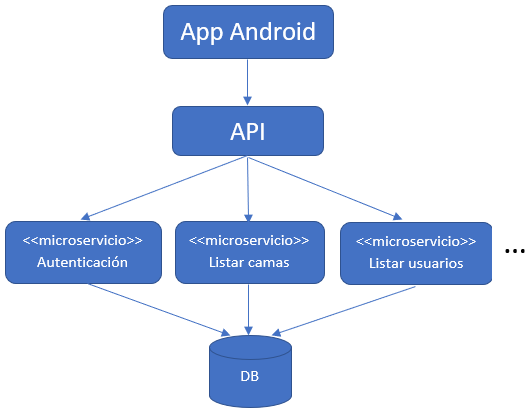
\includegraphics[width=0.8\textwidth]{../img/microservicios.png}
	\caption{Resumen de la arquitectura de microservicios.}
	\label{fig:microservicios}
\end{figure}

\subsection{Comunicación con la API}

Como se expone detenidamente en el apéndice de Especificación de requisitos, la aplicación ofrecerá, a grandes rasgos, tres funcionalidades principales: 

\begin{enumerate}
	\item \textbf{Gestión de usuarios:} permite gestionar qué usuarios y con qué credenciales pueden acceder al sistema. Esta funcionalidad solo estará disponible para el usuario con rol de admnistrador. 
	\item \textbf{Gestión de camas:} permite gestionar las camas instaladas y qué usuarios tienen acceso a sus datos. También estará disponible solo para el usuario administrador. 
	\item \textbf{Visualización de camas:} permite visualizar en tiempo real los datos captados por las camas a las que el usuario tiene acceso. El usuario administrador tendrá acceso a todas las camas instaladas, el resto solo a las especificadas por el administrador. 
\end{enumerate}

Todas estas funcionalidades se basan en los servicios disponibles en la API de mi compañero. Las especificaciones de la API se exponen en el Manual del programador contenido en los anexos de su trabajo, donde se explica que se distingue entre dos tipos de comunicación: 

\begin{enumerate}
	\item La mayor parte de los servicios se basan en peticiones POST a rutas específicas en función del servicio. Este tipo de comunicación abarca servicios de autentificación, consulta y modificación de datos de gestión (tanto de usuarios como de camas). 
	\item De forma particular, el sistema que proporciona los datos captados por las camas en tiempo real se maneja a través de mensajes entre \textit{WebSockets} usando la librería Socket.IO. 
\end{enumerate}

\subsubsection{Peticiones POST}
Dado que el funcionamiento de la aplicación depende casi enteramente de la comunicación con la API, debemos estar seguros de que existe conexión antes de realizar cada petición POST. Además, tal y como se implementa la API, un usuario solo puede mantener la autentificación en un dispositivo al mismo tiempo, de forma que, si el usuario <<alicia>> entra al sistema desde un dispositivo, y posteriormente lo hace desde otro, solo mantendrá la autentificación desde este último y perderá las credenciales desde el primero. Para gestionar estos dos problemas se define el siguiente esquema general de comunicación para cada petición POST:  

\begin{minipage}{\linewidth}
\begin{enumerate}
	\item Se comprueba que existe conexión a internet.
	\begin{enumerate}
		\item Si existe se continúa. 
		\item Si no existe se espera a recuperar la conexión o se pregunta al usuario si desea volver a la pantalla de inicio. 
	\end{enumerate}
	\item Se comprueba que el usuario sigue teniendo credenciales en el sistema.
	\begin{enumerate}
		\item Si es así se continúa. 
		\item Si no, se muestra un mensaje comunicando que se ha abierto sesión desde un dispositivo distinto y se redirige a la pantalla de inicio. 
	\end{enumerate}
	\item Se realiza la petición POST
	\begin{enumerate}
		\item Si la respuesta es satisfactoria se refleja el resultado en la interfaz o se indica que la operación se ha llevado a cabo con éxito.  
		\item Si la respuesta no es satisfactoria pero no se debe a un error del servidor, se muestra un mensaje de error al usuario. 
		\item Si la respuesta no es satisfactoria debido a un error del servidor se muestra un mensaje de error y se redirige a la pantalla de inicio. 
	\end{enumerate}
\end{enumerate}
\end{minipage}

Además, se tomó la decisión de que cada petición a la API, tanto POST como mediante WebSockets para la recepción de mensajes en tiempo real, se gestione por un hilo independiente. De esta forma se pueden recibir y mostrar datos de varias camas al mismo tiempo de forma sencilla y transparente. 

\subsubsection{Comunicación en tiempo real con \textit{Socket.IO}}

Al emplear esta biblioteca en la API, también debe usarse en el cliente para que la comunicación en tiempo real sea efectiva. 

A rasgos generales la comunicación se realiza en dos pasos: 

\begin{enumerate}
	\item Se conecta un \textit{Socket} a la ruta genérica del servidor y se emite un evento <<give\_me\_data>>. 
	\item Se conecta otro \textit{Socket} a la ruta formada por por la concatenación de la ruta genérica y el namespace que identifica la cama que se desea escuchar. A través de este \textit{Socket} se recibirán los eventos <<package>> con los datos en tiempo real. 
\end{enumerate}

\subsection{Autenticación}

La autenticación se resuelve de una forma muy sencilla desde el servidor. La primera petición POST que se debe realizar es la de autenticación, que recibe un nombre de usuario y una contraseña. Si el usuario tiene permiso para acceder al sistema, recibe un \textit{token} que se guarda como variable de sesión. Todas las peticiones POST sucesivas recibirán como parámetro este \textit{token}. 

\subsection{Actualización de la interfaz en tiempo real}

Para la funcionalidad de visualización de camas, la aplicación va a recibir continuamente los datos captados por la cama en tiempo real, y queremos que la interfaz se actualice cada vez que llega un dato. 

Dado que es un hilo el que gestiona la recepción de datos en tiempo real, para que la interfaz de usuario se actualice cada vez que se recibe un dato necesitamos implementar un mecanismo que permita que el hilo se lo notifique. La solución más sencilla que puede venir a la mente es el uso de un patrón observador. 

\begin{figure}[H]
	\centering
	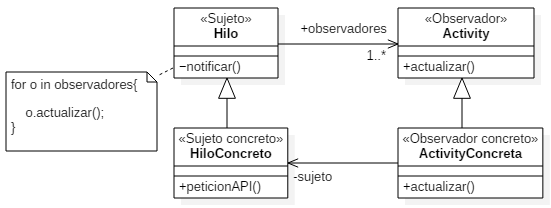
\includegraphics[width=1\textwidth]{../img/observador.png}
	\caption{Posible aplicación del patrón observador.}
	\label{fig:observador}
\end{figure}

Según se muestra en la figura~\ref{fig:observador}, la interfaz (Activity) tendría una referencia al hilo que realiza la petición, el que a su vez tendría una referencia a la interfaz. Desde su referencia a la interfaz, el hilo podría ejecutar el método \texttt{actualizar()}.

Esta es una solución muy simple y efectiva para muchas plataformas, pero no funciona en el caso de Android, ya que la actualización de los elementos de la interfaz (\textit{Layouts}) solo se puede realizar desde el hilo principal. Al llamar al método \texttt{actualizar()} desde el hilo, saltaría una excepción si dentro de este método se manipula algún elemento de la interfaz. 

Android ofrece varias alternativas para abordar este problema, y en mi caso he usado la que me ha parecido más sencilla: \textbf{el uso de \textit{Handlers}}~\cite{handler}. La idea es la misma, pero en este caso el \textit{Activity} tiene una referencia a un objeto \textit{Handler} que contiene el método \texttt{handleMessage}, el cual será el encargado de actualizar la interfaz. Cuando el \textit{Activity} lanza el hilo, le pasa la referencia al objeto \textit{Handler} como argumento. Cuando el hilo reciba un nuevo dato, se lo notificará ejecutando el método \texttt{sendMessage} del \textit{Handler}. Esta llamada activará el método \texttt{handleMessage}, que a diferencia del método \texttt{actualizar} del patrón observador, sí se ejecuta en el hilo principal. 

\section{Aspectos relevantes generales}

Este proyecto se me asignó gracias a la concesión de la \textbf{beca de colaboración de estudiantes en departamentos universitarios}, en este caso el departamento de Ingeniería Civil. Esta beca tiene como objetivo la implicación del estudiante en un proyecto de investigación, ofreciendo la posibilidad de ampliar sus conocimiento y concretar sus intereses para la posible incorporación a futuras tareas docentes o investigadoras. 

La realización de este proyecto me ha permitido experimentar a grandes rasgos en qué consiste la labor de un investigador, y la experiencia, definitivamente, me ha llevado a considerar muy positivamente esta salida laboral. 



\capitulo{6}{Trabajos relacionados}

Como ya se ha comentado, al inicio del proyecto se realizó una exploración inicial del estado del arte sobre detección automática de ataques epilépticos y otros problemas aplicables, como la detección de caídas. En este apartado se van a exponer los artículos más relevantes y aquellos que se centraban más en técnicas aplicables a nuestro problema concreto. 

\section{Revisión de técnicas}

Uno de los artículos más interesantes y que más información aportó fue \textbf{\textit{Seizure detection, seizure prediction, and closed-loop warning systemsin epilepsy}}~\cite{ramgopal2014epilepsy}, que realiza una revisión de los artículos más relevantes sobre el tema hasta 2014. En base a los artículos revisados, se expone el conjunto de técnicas utilizadas para la extracción de datos, abarcando desde electroencefalogramas (\textit{EEG}), electrocardiogramas (\textit{ECG}), acelerometría en dispositivos portátiles, sistemas de detección de vídeo y matrices de sensores de presión. Además, para cada artículo, se menciona la técnica de detección utilizada y finalmente una lista de compañías que comercializan los dispositivos de detección existentes. 

En el conjunto general de técnicas destacan la detección automática mediante \textit{EEG} y la detección basada en datos biométricos captados mediante diversos dispositivos, por ser los más usados y los que parecen ofrecer mejores rendimientos.  

Cabe destacar que aunque sí se menciona la existencia de dispositivos basados en matrices de sensores de presión, no se aporta ningún artículo en el que se expongan los métodos usados para lograr la detección de crisis mediante los datos recogidos de esta forma. 

\section{Detección de crisis mediante electroencefalograma}

Dentro de los artículos que hacían referencia al uso de electroencefalogramas, el que nos ha resultado más interesante es \textbf{\textit{Automated Epileptic Seizure Detection Methods: A Review
Study
}}~\cite{tzallas2012automated}, ya que enumera y explica las técnicas de detección de picos de señal más utilizadas. Sin embargo, aunque resulta interesante para ver distintas formas de tratar con datos en forma de señal, ninguna de ellas es directamente aplicable a nuestro problema, ya que el tipo de datos con los que trabaja son completamente distintos. 

\section{Detección de crisis mediante \textit{wearables}}

Según el artículo de revisión mencionado~\cite{ramgopal2014epilepsy}, otra de las técnicas más usadas para la recogida de datos para detección de crisis es la acelerometría aplicada a dispositivos portátiles como pulseras, o en la captación de constantes vitales a partir de pulseras y aparatos integrados en un parche pensado para colocarse en la zona del pecho. 

En un principio, esta línea de trabajo sí nos resultó interesante, ya que nuestro conjunto de datos original contaba con datos relativos a las constantes vitales del paciente, pero como ya se ha explicado, la calidad de esos datos era demasiado mala y hubo que desecharlos en la fase de preprocesado. 

\section{Detección mediante presiones y otros problemas aplicables}

Otra técnica interesante encontrada, no necesariamente aplicada a la detección de crisis epilépticas, fue la estimación de la frecuencia respiratoria y la frecuencia cardíaca a partir de datos de presión. Esto, a priori, podría ayudarnos a abordar nuestro problema de falta de datos de los ese tipo, pero como se deduce de las explicaciones de artículos~\cite{kortelainen2012, guerreromora2012}, la precisión de los sensores de presión con los que trabajamos nosotros no es en absoluto suficiente. 

Por último, y dado que no se encontraron referencias a métodos concretos de aplicación de matrices de presión para la detección de crisis epilépticas, se exploró una línea de trabajo distinta, centrada en la detección de caídas mediante datos de presión, que aunque no tratara el mismo tipo de problema, los métodos de trabajo aplicados podrían servirnos de referencia para el nuestro. Uno de los artículos encontrados~\cite{huanwen2010} trabaja con datos de presión tomados desde el suelo y datos de imagen infrarroja, el otro~\cite{tolkiehn2011} trabaja con un acelerómetro y datos extraídos de un sensor de presión barométrica. 

Aunque finalmente ninguna de estas líneas sirvió como punto de partida para nuestro proyecto, la exploración del estado del arte nos proporcionó una visión general de las técnicas más usadas y su precisión. 



\capitulo{7}{Conclusiones y Líneas de trabajo futuras}

Todo proyecto debe incluir las conclusiones que se derivan de su desarrollo. Éstas pueden ser de diferente índole, dependiendo de la tipología del proyecto, pero normalmente van a estar presentes un conjunto de conclusiones relacionadas con los resultados del proyecto y un conjunto de conclusiones técnicas. 
Además, resulta muy útil realizar un informe crítico indicando cómo se puede mejorar el proyecto, o cómo se puede continuar trabajando en la línea del proyecto realizado. 



\bibliographystyle{plain}
\bibliography{bibliografia}

\end{document}
